%% LyX 2.1.4 created this file.  For more info, see http://www.lyx.org/.
%% Do not edit unless you really know what you are doing.
\documentclass[british,english,a4paper,12pt,numbered,times,online]{PhDThesisLyX}
\usepackage[T1]{fontenc}
\usepackage[latin9]{inputenc}
\usepackage{geometry}
\geometry{verbose,tmargin=1in,bmargin=1in,lmargin=1.25in,rmargin=1in}
\setcounter{secnumdepth}{3}
\setcounter{tocdepth}{3}
\usepackage{verbatim}
\usepackage{prettyref}
\usepackage{amstext}
\usepackage{amsthm}
\usepackage{cancel}
\usepackage{makeidx}
\makeindex
\usepackage{graphicx}
\usepackage{setspace}
\onehalfspacing

\makeatletter

%%%%%%%%%%%%%%%%%%%%%%%%%%%%%% LyX specific LaTeX commands.

\let\pr@chap=\pr@cha

%%%%%%%%%%%%%%%%%%%%%%%%%%%%%% Textclass specific LaTeX commands.
 \theoremstyle{definition}
 \newtheorem*{defn*}{\protect\definitionname}
  \theoremstyle{plain}
  \newtheorem*{prop*}{\protect\propositionname}

%%%%%%%%%%%%%%%%%%%%%%%%%%%%%% User specified LaTeX commands.

%%%%%%%%%%%%%%%%%%%%%%%%%%%%%%%%%%%%%%%%%%%%%%%%%%%%%%%%%%%%%%%%%%%%%%%%%%%%%%%%
%%                                                                            %%
%% Class ``PhD Thesis LyX''                                                   %%
%%                                                                            %%
%% A PhD thesis LyX template for Cambridge University Engineering Department  %%
%%                                                                            %%
%% Version: v1.0                                                              %%
%% Authors: Krishna Kumar                                                     %%
%% Date: 10/01/2014 (inception)                                               %%
%% License: MIT License (c) 2014 Krishna Kumar                                %%
%% GitHub Repo: https://github.com/kks32/PhDThesisLyX			      %%
%%%%%%%%%%%%%%%%%%%%%%%%%%%%%%%%%%%%%%%%%%%%%%%%%%%%%%%%%%%%%%%%%%%%%%%%%%%%%%%%
%\usepackage{hyperref}
\usepackage{url}
\title{Contextuality in a Deterministic Quantum Theory}
\authorprefix{Mr.}
\author{Atul Singh Arora}
\regno{MS11003}
\dept{Department of Physical Sciences}
\university{Indian Institute of Science Education and Research, Mohali}
\crest{
\includegraphics[width=0.25\textwidth]{Figs/IISER_Mohali_Logo_2014}}
\degree{Master of Science}
\college{IISER Mohali}
\degreedate{April 22, 2016}
\guide{Prof. Arvind}
\guidedeclare{In my capacity as the supervisor of the candidate's project work, I certify that the aforesaid statements by the candidate are true to the best of my knowledge.}
\panela{Dr. Abhishek Choudhuri}
\panelb{Dr. Kamal P. Singh}
\certificatetext{This is to certify that the dissertation titled \textbf{\@title{}}, submitted by \textbf{\@authorprefix{} \@author{}} (Registration Number: \@regno{}) for the partial fulfilment of the BS-MS dual degree programme of the \@university{}, has been examined by the thesis committee duly appointed by the institute. The committee finds the work done by the candidate satisfactory and recommends that the report be accepted.}

\@ifundefined{showcaptionsetup}{}{%
 \PassOptionsToPackage{caption=false}{subfig}}
\usepackage{subfig}
\makeatother

\usepackage{babel}
  \addto\captionsbritish{\renewcommand{\definitionname}{Definition}}
  \addto\captionsbritish{\renewcommand{\propositionname}{Proposition}}
  \addto\captionsenglish{\renewcommand{\definitionname}{Definition}}
  \addto\captionsenglish{\renewcommand{\propositionname}{Proposition}}
  \providecommand{\definitionname}{Definition}
  \providecommand{\propositionname}{Proposition}

\begin{document}
\begin{comment}
\textbf{Cambridge University Engineering Department Thesis Template
ported to \LyX{}2.0 }

Author: Krishna Kumar

Distributed under MIT License.

Website: https://github.com/kks32/PhDThesis\LyX{}

{*}{*}{*}{*}{*}{*}{*}{*}{*}{*}{*}{*}{*}{*}{*}{*}{*}{*}{*}{*}{*}{*}{*}{*}{*}{*}{*}{*}{*}{*}{*}{*}{*}{*}{*}{*}{*}{*}{*}{*}{*}{*}{*}{*}{*}{*}{*}{*}{*}{*}{*}{*}{*}{*}{*}{*}{*}{*}{*}{*}{*}{*}{*}{*}{*}{*}{*}{*}{*}{*}{*}{*}{*}{*}{*}{*}{*}{*}{*}{*}{*}{*}{*}{*}{*}{*}{*}{*}{*}{*}{*}{*}{*}{*}{*}{*}{*}{*}{*}{*}{*}{*}{*}{*}{*}{*}{*}{*}{*}{*}{*}{*}

\textbf{Thesis Information}

Go to \textsf{Document > Settings > \LaTeX{} preamble} to modify the
\textsf{title, author, year, department} fields.

{*}{*}{*}{*}{*}{*}{*}{*}{*}{*}{*}{*}{*}{*}{*}{*}{*}{*}{*}{*}{*}{*}{*}{*}{*}{*}{*}{*}{*}{*}{*}{*}{*}{*}{*}{*}{*}{*}{*}{*}{*}{*}{*}{*}{*}{*}{*}{*}{*}{*}{*}{*}{*}{*}{*}{*}{*}{*}{*}{*}{*}{*}{*}{*}{*}{*}{*}{*}{*}{*}{*}{*}{*}{*}{*}{*}{*}{*}{*}{*}{*}{*}{*}{*}{*}{*}{*}{*}{*}{*}{*}{*}{*}{*}{*}{*}{*}{*}{*}{*}{*}{*}{*}{*}{*}{*}{*}{*}{*}{*}{*}{*}

\textbf{Custom Options}

To set custom options supported by the class file go to Document >
Settings > Document class and enter \textbf{``a4paper,12pt,numbered,oneside,print}''
without quotes in the custom field.

\textbf{Paper Size}: a4paper / a5paper

`a4paper'(The University of Cambridge PhD thesis guidelines recommends
a4 page size - default option) or `a5paper': A5 Paper size is also
allowed as per the Cambridge University Engineering Deparment guidelines
for PhD thesis 

\textbf{FontSize: }10pt / 11pt / 12pt

`11pt' or `12pt'(default): Font Size 10pt is NOT recommended by the
University guidelines 

\textbf{Layout: }`\textbf{oneside}' or `\textbf{twoside}'(default):
Printing double side (twoside) or single side.

\textbf{Mode (print / online)}: Use `print' for print version with
appropriate margins and page layout. Leaving the options field blank
will activate Online version. 

\textbf{draft}: For draft mode without loading any images (same as
draft in book) 

{*}{*}{*}{*}{*}{*}{*}{*}{*}{*}{*}{*}{*}{*}{*}{*}{*}{*}{*}{*}{*}{*}{*}{*}{*}{*}{*}{*}{*}{*}{*}{*}{*}{*}{*}{*}{*}{*}{*}{*}{*}{*}{*}{*}{*}{*}{*}{*}{*}{*}{*}{*}{*}{*}{*}{*}{*}{*}{*}{*}{*}{*}{*}{*}{*}{*}{*}{*}{*}{*}{*}{*}{*}{*}{*}{*}{*}{*}{*}{*}{*}{*}{*}{*}{*}{*}{*}{*}{*}{*}{*}{*}{*}{*}{*}{*}{*}{*}{*}{*}{*}{*}{*}{*}{*}{*}{*}{*}{*}{*}{*}{*}

\textbf{Bibliography style: }

To define document class options like bibliography style (\textbf{numbered}
/ \textbf{authoryear}) go to Document > Settings > Document classs
and enter ``numbered'' or ``authoryear'' without quotes in the
custom field.

{*}{*}{*}{*}{*}{*}{*}{*}{*}{*}{*}{*}{*}{*}{*}{*}{*}{*}{*}{*}{*}{*}{*}{*}{*}{*}{*}{*}{*}{*}{*}{*}{*}{*}{*}{*}{*}{*}{*}{*}{*}{*}{*}{*}{*}{*}{*}{*}{*}{*}{*}{*}{*}{*}{*}{*}{*}{*}{*}{*}{*}{*}{*}{*}{*}{*}{*}{*}{*}{*}{*}{*}{*}{*}{*}{*}{*}{*}{*}{*}{*}{*}{*}{*}{*}{*}{*}{*}{*}{*}{*}{*}{*}{*}{*}{*}{*}{*}{*}{*}{*}{*}{*}{*}{*}{*}{*}{*}{*}{*}{*}{*}

\textbf{Page Style}

`\textbf{default (leave empty)}': For Page Numbers in Header (Left
Even, Right Odd) and Chapter Name in Header (Right Even) and Section
Name (Left Odd). Blank Footer. 

\textbf{`PageStyleI'}: Chapter Name next \& Page Number on Even Side
(Left Even). Section Name \& Page Number in Header on Odd Side (Right
Odd). Footer is empty. 

\textbf{`PageStyleII'}: Chapter Name on Even Side (Left Even) in Header.
Section Number \% and Section Name in Header on Odd Side (Right Odd).
Page numbering in footer 

{*}{*}{*}{*}{*}{*}{*}{*}{*}{*}{*}{*}{*}{*}{*}{*}{*}{*}{*}{*}{*}{*}{*}{*}{*}{*}{*}{*}{*}{*}{*}{*}{*}{*}{*}{*}{*}{*}{*}{*}{*}{*}{*}{*}{*}{*}{*}{*}{*}{*}{*}{*}{*}{*}{*}{*}{*}{*}{*}{*}{*}{*}{*}{*}{*}{*}{*}{*}{*}{*}{*}{*}{*}{*}{*}{*}{*}{*}{*}{*}{*}{*}{*}{*}{*}{*}{*}{*}{*}{*}{*}{*}{*}{*}{*}{*}{*}{*}{*}{*}{*}{*}{*}{*}{*}{*}{*}{*}{*}{*}{*}{*}

\textbf{Font}

`\textbf{times}`: (The University of Cambridge guidelines recommend
using Times). Specifying times option in the document class will use
`mathptpx` or `Times` font with Math Support. 

`\textbf{fourier}`: fourier font with math support

`\textbf{default (empty)}`: When no font is specified, `Latin Modern`
is used as the default font with Math Support. 

Go to Document > Settings > Document class and include `times` or
`fourier` in the custom field.
\end{comment}


% Title Page
\begin{romanpages}
\begin{titlepage}
\maketitle
\end{titlepage}
% FrontMatter

\begin{dedication}
I would like to dedicate this thesis to my mother, who introduced
me to the most valuable notion, that of freedom, and to my father
who fostered it.\end{dedication}



\begin{declaration}
I hereby declare that except where specific reference is made to the
work of others, the contents of this dissertation are original and
have not been submitted in whole or in part for consideration for
any other degree or qualification in this, or any other University.
This dissertation is the result of my own work and includes nothing
which is the outcome of work done in collaboration, except where specifically
indicated in the text.

\begin{comment}
This dissertation contains fewer than 65,000 words including appendices,
bibliography, footnotes, tables and equations and has less than 150
figures.
\end{comment}
\end{declaration}



\begin{certificate}
\end{certificate}



\begin{acknowledgements}
I acknowledge the contribution of my project guide, Prof. Arvind,
who provided me with an environment conducive to research, and motivation
to facilitate completion of this project. He encouraged independent
thinking and guided me through difficulties I encountered.

Discussions with the Quantum Computation \& Quantum Information (QCQI)
group members, especially those with Rajendra Bhati and Kishor Bharti
have been particularly efficacious. Inputs from Jaskaran Singh have
also been helpful. The QCQI group seminars, specifically, those by
Samridhi Gambhir and Dr. Arun Shehrawat, have helped narrowing the
thesis problem. 

Dr. Abhishek Choudhuri and Prof. Sudeshna Sinha, although formally
not related to the project, have been kind enough to assist me at
various instances with challenges I faced while numerically simulating
the equations. 

I am grateful to my parents and my colleagues/friends, who have been
pivotal to helping me maintain mental balance, inspired me and provided
emotional support, in ways they perhaps don't realize, specifically
Manu Jayadharan, Prashansa Gupta, Kishor Bharti, Ritu Roy Chowdhury,
Vivek Sagar, Yosman BapatDhar, Saumya Gupta, Shwetha Srinivasan, Evelyn
Abraham and Srijit Mukherjee.

I end with acknowledging Immanuel Kant, for his philosophical work
on ethics, which has heavily affected my thoughts, actions and outlook
to life.\selectlanguage{english}%
\end{acknowledgements}



\begin{abstract}
The Copenhagen Interpretation of Quantum Mechanics (QM) asserts that
the wavefunction is the most complete description, which entails that
there is an inherent fuzziness in our description of nature. There
exists a completion of QM, known as Bohmian Mechanics (BM), which
replaces this fuzziness with precision, and re-introduces notions
of physical trajectories. Various interesting questions arise, solely
by existence of such a description; doesn't it contradict the uncertainty
principle, for instance. Most of these questions were found to have
been addressed satisfactorily in the literature. There was however,
one question, whose answer has become the subject of the thesis; that
of the paradoxical co-existence of contextuality and BM. In a theory
that can predict the value of operators, the value an operator takes,
must depend on the state of the system (including hidden variables).
Contextuality arguments show that the value an operator takes, must
also depend on the complete set of compatible operators, to be consistent
with QM. BM being deterministic, is at complete odds with this notion. 

After various attempts we were able to show, that the notion of contextuality
is infact not necessary. This was achieved by identifying another
`classical property' and constructing a non-contextual toy-model,
serving as a counter-example to the impossibility proof. The toy model
has been generalized to a discrete but arbitrarily sized Hilbert space,
consistent with all predictions of QM. Implications of violation of
this `classical property' have been discussed, in particular, to the
notion of non-locality.

\begin{comment}
given the physical situation (including hidden variables) and the
state, can predict the value of any operator; the prediction doesn't
depend on anything else.
\end{comment}
\end{abstract}



% List of Contents, Figures and Tables

\tableofcontents{}

\listoffigures


\begin{comment}
\listoftables
\end{comment}


% To print nomenclature
% \printnomenclature[space] %space can be set as 2.5cm between symbol and description
% \printnomencl
\end{romanpages}
% Main matter
\setcounter{page}{1}

\selectlanguage{british}%

\chapter{Prologue}


\section{Overview}

A course in Quantum Mechanics (QM) typically leaves the reader with
a fuzzy view of the world. The founders of the subject, were able
to abstract out the mathematics from it's implications and interpretation.
The view that the wavefunction is the most complete description of
a system, known as the `Orthodox Copenhagen Interpretation', is among
the most popular. Einstein and Bohm, both played an important role
in challenging this belief. \\
Einstein showed \cite{EinsteinEPR} that if one makes reasonable assumptions
about nature (in the spirit of his relativity theories), then QM must
be incomplete. By incompleteness, he meant that the results of certain
experiments should be predictable precisely, but QM fails at doing
this. Thus he concluded that, QM must be treated as an intermediate
theory and that a more complete description of nature should be sought.
We will come back to this discussion. \\
Bohm challenged this view by realizing that one can't experimentally
refute the interpretation. His argument was that if for instance,
the predictions of QM fail to match with experiments, then one can
always add appropriate terms in the Hamiltonian until the difficulty
is resolved. He was already anticipating the modern form of particle
physics. To accurately account for interactions between particles,
one can postulate new force mediating particles, which was also done
in the history of the subject. However, one can't refute the interpretation
on grounds of inaccuracy in predictions. He therefore, aimed at, and
succeeded at constructing a complete quantum theory \cite{Bohm1},
now known as Bohmian Mechanics (BM)\footnote{Historically, Louis de Broglie had proposed a similar construction,
but abandoned the idea soon after. Bohm established it to be a consistent
theory.}. Its existence showed that we are not justified at believing the
interpretation, simply because there exists at least one alternative.

Returning to Einstein, %
\begin{comment}
as will be described in more detail
\end{comment}
Bell was able to construct a physical situation, that would test the
very requirements Einstein imposed on a complete quantum theory; he
was able to show that according to predictions of QM, \emph{such}
a complete description is impossible. This was verified experimentally
\cite{BellExp72,BellExpAspect81} (and was confirmed to be true, without
any possible loop-holes \cite{BellExpHensen2015}, only in 2015).\\
It might appear that Bell's test shows that QM is inconsistent with
BM. Upon looking at the details however, one can be convinced, that
this is not the case. Infact, Bell was among the first few to popularize
BM \cite{BellSpeakable}.

The discussion so far, is well known in the literature. However, certain
developments which followed the said work of Bohm, again lead to apparent
inconsistencies between BM and QM. These had not been satisfactorily
addressed in the literature and have become the subject of this thesis.
\\
For the sake of completeness, we merely name these. One must look
at the details, to be able to appreciate them. Greenberger, Horne
and Zeilinger (GHZ), constructed a test \cite{GHZ} that apparently
showed determinism can't exist, i.e. the notion that observables have
pre-defined values is inconsistent with QM. Developments due to Gleason
\cite{Gleason}, Bell himself \cite{BellOnHiddenVariables}, Kochen,
Specker \cite{KochenSpecker}, Peres and Mermin \cite{Peres,Mermin},
showed that the value an operator takes, must depend on the context
in which it is measured; context here refers to the complete set of
compatible operators.\\
The apparent contradiction must now be clear; BM is deterministic
and it is at odds with the notion of contextuality as well. 

\begin{comment}
\nomenclature{E}{Energy}\nomenclature{$m_0$}{intrinsic rest mass}\nomenclature{c}{speed of light}\nomenclature{p}{momentum}
\end{comment}



\section{The EPR argument}

%\begin{multicols}{3}

The EPR argument requires an entangled state, over two particles,
which was originally written as 
\[
\psi(q_{1},q_{2})=\int e^{-i(q_{1}-q_{2}+q_{0})p/\hbar}dp=\delta(q_{1}-q_{2}+q_{0}).
\]
In the modern notation, one can write this as 
\begin{eqnarray*}
\left|\psi\right\rangle  & = & \int\delta(q_{1}-q_{2}+q_{0})dq_{1}dq_{2}\left|q_{1}\right\rangle _{A}\left|q_{2}\right\rangle _{B}\\
 & = & \int\left|q\right\rangle _{A}\left|q+q_{0}\right\rangle _{B}dq.
\end{eqnarray*}
Similarly, one can write the same state as 
\begin{eqnarray*}
\left|\psi\right\rangle  & = & \int e^{-i(q_{1}-q_{2})p/\hbar}dpdq_{1}dq_{2}\left|q_{1}\right\rangle _{A}\left|q_{2}\right\rangle _{B}\\
 & = & \int e^{-iq_{1}p/\hbar}\left|q_{1}\right\rangle _{A}dq_{1}e^{iq_{2}p/\hbar}\left|q_{2}\right\rangle _{B}dq_{2}dp\\
 & = & \int\left|p\right\rangle _{A}\left|-p\right\rangle _{B}dp.
\end{eqnarray*}
where $A$ and $B$ label the particles. An attempt to reproduce the
precise argument, will not be made. Instead, we satisfy ourselves
with the following simplified argument. We assume the principle of
locality holds, which is to say that if two particles are sufficiently
far away, then any change made to one particle, should not influence
the other instantaneously. Given this assumption, consider two particles,
which are sufficiently far away and that their state is given by $\left|\psi\right\rangle $.
Now if the momentum of particle $B$ is measured by observer $B$,
then observer $B$, according to QM, will be able to predict the momentum
of particle $A$. Similarly, if the position of particle $B$ is measured,
then observer $B$ can predict the position of particle $A$. Further,
note that the choice made by observer $B$, can't influence particle
$A$, by the assumption of locality. It therefore follows that particle
$A$ had both it's position and momentum well defined, without being
measured. QM fails to yield the answer with precision, whereas as
we have shown, the answer was precise. Thus, we are forced to conclude
that QM is not a complete description of nature.

Einstein ended his paper with this remark: ``While we have thus shown
that the wave function does not provide a complete description of
the physical reality, we left open the question of whether or not
such a description exists. We believe, however, that such a theory
is possible.'' \cite{EinsteinEPR}


\section{Bell's Theorem\label{sec:Bell's-Theorem}}

Bell's work addresses and satisfactorily answers Einstein's open question,
of whether a \emph{such} a description exists. Consider the following
scenario. There are two observers, A and B, each has a particle. Each
observer, can measure two properties, call them $\hat{a}_{1},\hat{a}_{2}$
for observer A and $\hat{b}_{1},\hat{b}_{2}$ for observer B, which
yield a $\pm1$ outcome. Let $\left\langle \hat{a}_{i}\hat{b}_{j}\right\rangle $
represent the average value obtained by measuring the property $\hat{a}_{i}$
and $\hat{b}_{j}$ on the first and second particle respectively.
Consider the average given by $\left\langle \hat{B}\right\rangle =\left\langle \hat{a}_{1}\hat{b}_{1}\right\rangle +\left\langle \hat{a}_{1}\hat{b}_{2}\right\rangle +\left\langle \hat{a}_{2}\hat{b}_{1}\right\rangle -\left\langle \hat{a}_{2}\hat{b}_{2}\right\rangle $.
If one assumes local realism\footnote{Infact, an argument similar to EPR can be used to show that locality
entails realism.}, that is that the values $a_{i}$ takes are unaffected by those taken
by $b_{i}$ and that $\hat{a}_{i},\hat{b}_{j}$ have pre-defined values
(respectively), then $\left\langle \hat{B}\right\rangle \le2$. One
can check this quickly by a brute force substitution of $\pm1$ values,
in place of $a_{i},b_{j}$.

Consider now, the state $\left|\psi\right\rangle =\left(\left|+-\right\rangle -\left|-+\right\rangle \right)/\sqrt{2}$,
where $\hat{\sigma}_{x}\left|\pm\right\rangle =\pm\left|\pm\right\rangle $,
and $\hat{\sigma}_{x,y,z}$ are the Pauli matrices, given in the z-basis
as 
\[
\hat{\sigma}_{x}\doteq\left[\begin{array}{cc}
0 & 1\\
1 & 0
\end{array}\right],\,\hat{\sigma}_{y}\doteq\left[\begin{array}{cc}
0 & -i\\
i & 0
\end{array}\right],\,\hat{\sigma}_{z}\doteq\left[\begin{array}{cc}
1 & 0\\
0 & -1
\end{array}\right].
\]
Let $\hat{a}_{1}=\hat{\sigma}_{z}$ and $\hat{a}_{2}=\hat{\sigma}_{x}$,
while $\hat{b}_{1}=-\frac{\hat{\sigma}_{z}+\hat{\sigma}_{x}}{\sqrt{2}}$
and $\hat{b}_{2}=\frac{\hat{\sigma}_{z}-\hat{\sigma}_{x}}{\sqrt{2}}$.
Upon evaluating $\left\langle \hat{B}\right\rangle $ using the rules
of QM, one obtains $\left\langle \hat{B}\right\rangle =2\sqrt{2}\nleq2$.
This entails that our assumption, that of local realism, must be incorrect,
which settles the question: A \emph{local} hidden variable description
can not exist. The word hidden is used to represent information about
the state of the system, that is not contained in the wavefunction.
It is instructive to emphasize that a non-local description, may still
be possible. It is also important to note that, despite this non-locality,
one can't use QM to send signals instantaneously (superluminal communication
is not possible). This is known as the no-signalling theorem and can
be proven by showing that marginals in QM, don't depend on the system
which is traced out \cite{NielsenChuang}.


\section{Bohm's Theory, Bohmian Mechanics (condensed introduction)\label{sec:Bohm's-Theory,-Bohmian}}

Bohm gave a precise \cite{Bohm1}, but non-local description of quantum
phenomena. Let us start with non-interacting particles. A particle
is associated with (1) a position, $q$ \& momentum, $p$, precisely
defined and (2) a wavefunction $\psi=Re^{iS/\hbar}$. The postulates
of the theory are: (a) Evolution of the wavefunction, is governed
by Schrodinger's equation: $i\hbar\partial\psi/\partial t=-(\hbar^{2}/2m)\nabla^{2}\psi+V\psi$.
(b) The particle is guided by the wavefunction: $\dot{q}=p/m$ where
$p=\nabla S=\hbar\text{Im}(\nabla\psi/\psi)$. (c) The initial distribution
of the particles is given by $\rho(x)=\left|\psi\right|^{2}$.

The astute reader would've noticed that $\nabla S$ is just the probability
current, which entails that if the initial distribution satisfies
$\left|\psi(t_{0})\right|^{2}$, then it will do so at all times $t$,
thereafter. Before generalizing this to multiple particles, let us
first see a quick consequence of this formulation. In the Orthodox
Copenhagen interpretation, the double slit experiment is a source
of mystery and the which slit question, that of confusion. In BM,
since trajectories are well defined, one observes (see \prettyref{fig:Experimentally-observed-average})
that the particle goes through precisely one slit and then later,
forms the interference pattern. 
\begin{figure}
\begin{centering}
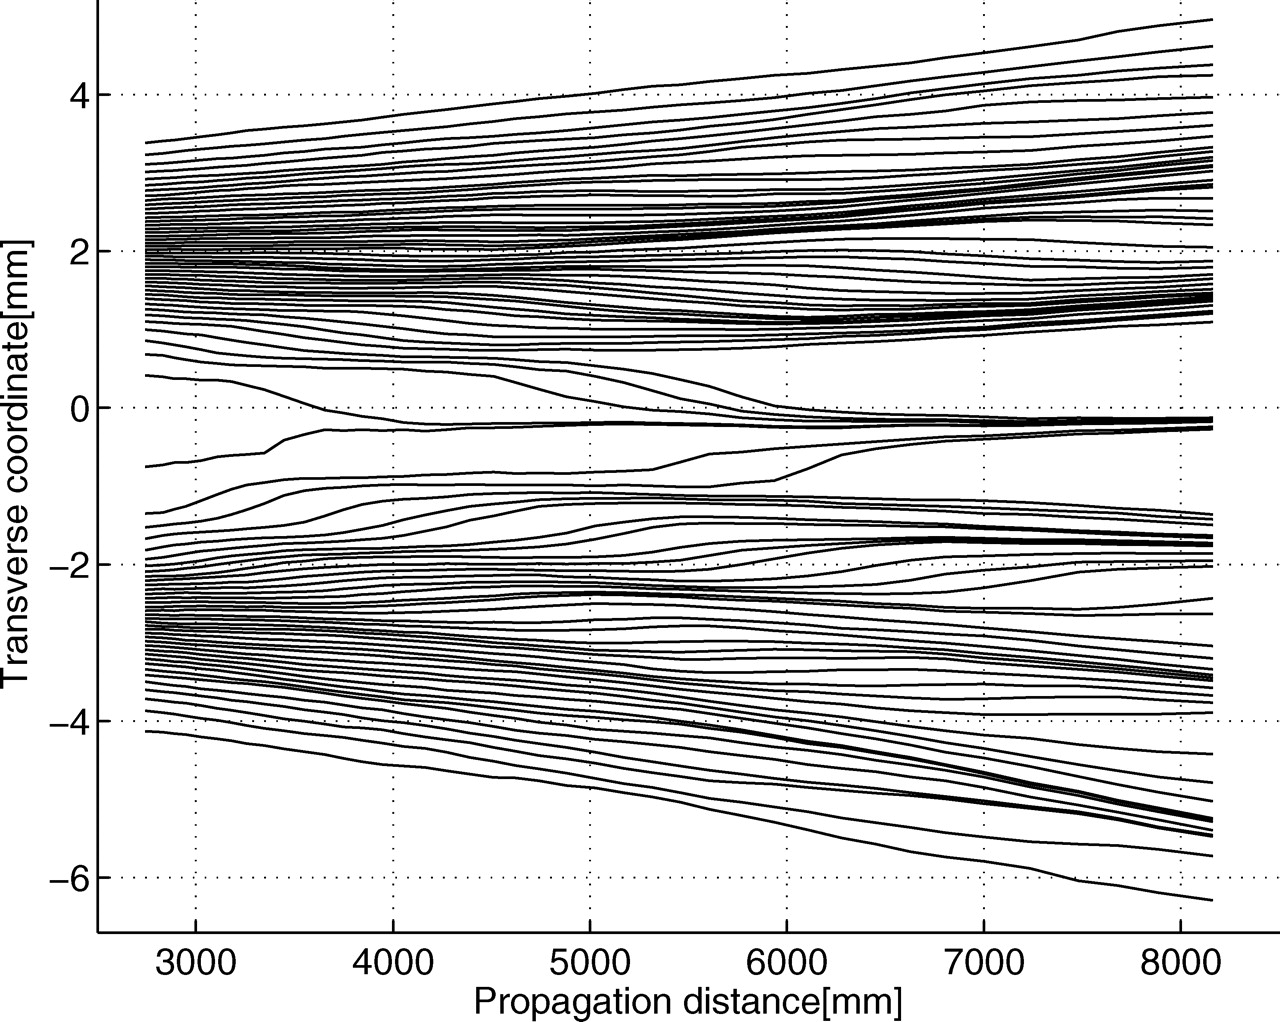
\includegraphics[width=0.7\textwidth]{Chapter1/Figs/Raster/singlePhotonTrajectory}
\par\end{centering}

\caption{Experimentally observed average single-photon trajectories. ``In
the case of single-particle quantum mechanics, the trajectories measured
in this fashion reproduce those predicted in the Bohm\textendash de
Broglie interpretation of quantum mechanics'' \cite{Kocsis1170}\label{fig:Experimentally-observed-average}}


\selectlanguage{english}%
\selectlanguage{english}%
\end{figure}
The wavefunction goes through both slits, and interferes to create
the pattern. If one of the slits is blocked, then since the wavefunction
can't interfere, the pattern is lost as expected. We haven't spoken
about measuring the particle yet, but if one notes that to measure
the particle, the potential at one of the slits must be changed, then
it is immediate that the interference pattern will be effected, since
the wavefunction is affected by the potential at both slits, even
if the particle passes through only one. One finds that by using the
following multi-particle generalization, and an appropriate measuring
scheme, one can show more precisely how the process of measuring effectively
destroys the pattern, replacing the mystery with clarity.

For $N$ interacting particles, we have $p_{i}=\nabla_{i}S(q_{1},q_{2},\dots,q_{N})$
where note that the momentum of the $i^{th}$ particle, depends on
the instantaneous positions of all the particles. Consequently, BM
is an explicitly non-local, but complete description. 

As a final remark, it must be added that spins can also be included
in BM, however, a particle is not associated with a specific spin,
only it's wavefunction is. For a spinor, say $\psi\equiv(\psi_{+},\psi_{-})^{T}$,
the generalization is that $p=\hbar\text{Im}((\psi,\nabla\psi)/(\psi,\psi))$
where $(.,.)$ represents inner product in the spin space $\mathbb{C}^{2}$.
A quick illustration is in order. Consider the following Stern-Gerlach
setup; Quantum effects are considered only along the $x$-axis. A
particle moves along the $z$-axis, with speed $v_{z}$, and it's
initial wavefunction, given by a Gaussian centred at the origin, say
$\psi(q_{x})=(1/\sqrt{2\pi}\sigma)e^{-q_{x}^{2}/2\sigma^{2}}$, viz.
$\left|\psi\right\rangle =\int dq\psi(q)\left|q\right\rangle $. It's
spin state is given by $\left|\chi\right\rangle =\left(\left|+\right\rangle +\left|-\right\rangle \right)/\sqrt{2}$,
where $\left|+\right\rangle $ and $\left|-\right\rangle $ are s.t.
$\sigma_{x}\left|\pm\right\rangle =\pm\left|\pm\right\rangle $. Along
the $z$-axis, a strong heterogeneous magnetic field is present, whose
action maybe captured by $H_{\text{int}}=a\hat{p}_{x}\otimes\hat{\sigma}_{x}$
where $a$ is a constant that quantifies the strength of the field.
Why this particular form works, will become clear momentarily. Assuming
that $a$ is large enough to neglect effects of free-evolution, we
have $\hat{U}(t)=e^{-ia\hat{p}_{x}\otimes\hat{\sigma}_{x}t/\hbar}$.
Thus, if the initial state is $\left|\Psi\right\rangle =\left|\psi\right\rangle \otimes\left|\chi\right\rangle $,
then 
\begin{eqnarray*}
\left|\Psi(t)\right\rangle  & = & \hat{U}(t)\left|\Psi\right\rangle \\
 & = & \frac{e^{-ia\hat{p}_{x}t/\hbar}\left|\psi\right\rangle \otimes\left|+\right\rangle +e^{ia\hat{p}_{x}t/\hbar}\left|\psi\right\rangle \otimes\left|-\right\rangle }{\sqrt{2}}\\
 & = & \frac{\left|\psi_{at}\right\rangle \otimes\left|+\right\rangle +\left|\psi_{-at}\right\rangle \otimes\left|-\right\rangle }{\sqrt{2}}
\end{eqnarray*}
where $\left|\psi_{q_{x0}}\right\rangle \equiv\int dq\psi(q_{x}-q_{x0})\left|q_{x}\right\rangle $,
viz. a Gaussian wavepacket centered at $q_{x0}$. One can plot $\left|\Psi\right|^{2}$,
as a function of $q_{z}$, using $q_{z}=v_{z}t$, schematically as
shown in the figure 
\begin{figure}
\begin{centering}
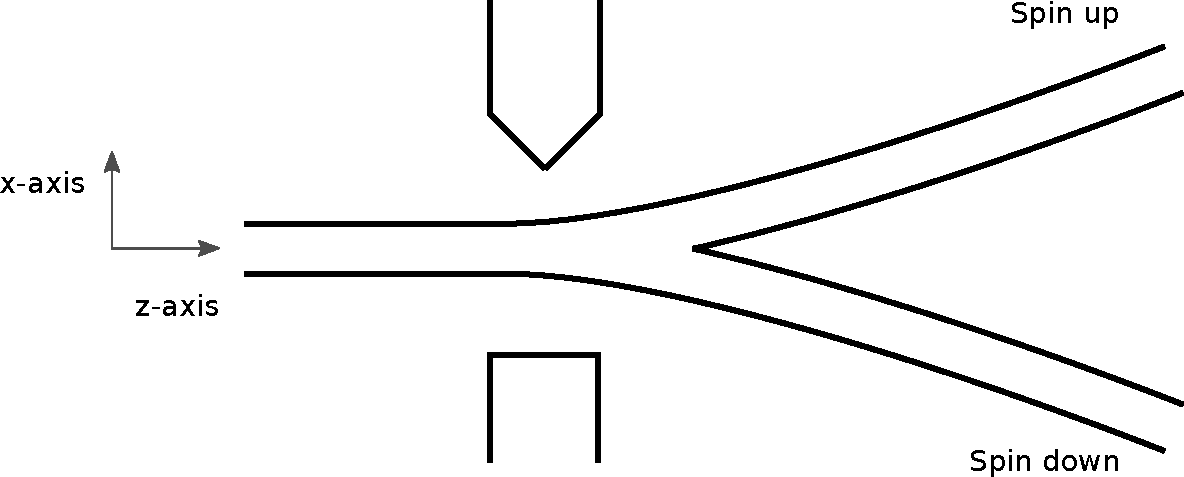
\includegraphics[width=0.8\textwidth]{Chapter1/Figs/Vectors/sg}
\par\end{centering}

\caption{Contour plot of $\left|\Psi(q_{x},t)\right|^{2}$ plotted for various
$t=q_{z}/v_{z}$, illustrating a Stern-Gerlach measurement. \label{fig:Contour-plot-of-Psi}}


\selectlanguage{english}%
\selectlanguage{english}%
\end{figure}
(see \prettyref{fig:Contour-plot-of-Psi}), where regions enclosing,
say $70\%$ of $\left|\Psi(q_{x})\right|^{2}$ have been outlined\footnote{Note that $\left|\Psi\right|^{2}=\left\langle \Psi|q_{x}\right\rangle \left\langle q_{x}|\Psi\right\rangle $,
where the spins are essentially traced over by the said expression}. So far, according to QM, if we measure the position of the particle,
then (given $\sigma\ll at$), obtaining the particle near $q_{x}=at$,
is as probable as finding it near $q_{x}=-at$. QM doesn't make a
deterministic prediction at this stage. According to BM, if in addition
to the wavefunction, we assume that the particle was initially at
some $q_{x}>0$, then we can predict precisely where the particle
will turn up. Infact, one can accomplish this with essentially no
calculation. Since $\dot{q}_{x}=\nabla S/m$, a single valued function,
it follows that trajectories of particles won't intersect, where recall
that $S$ is given by $\psi=Re^{iS/\hbar}$. Consequently, a particle
that starts with $q_{x}>0$, must follow the `up' trajectory, else
by symmetry, the trajectories will have to intersect. We conclude
therefore, that if $q_{x}>0$ initially, the particle has spin $\left|+\right\rangle $
and if $q_{x}<0,$ the spin must be $\left|-\right\rangle $. This
appears very clear and intuitive. A non-intuitive aspect of this,
is that we can't associate spins with particles, even though we can
predict precisely, the outcome of the experiment. This is manifested
by the observation that if $H_{\text{int}}\to-H_{\text{int}}$, which
practically amounts to reversing the heterogeneity of the magnet,
then $\sqrt{2}\left|\Psi(t)\right\rangle =\left|\psi_{-at}\right\rangle \otimes\left|+\right\rangle +\left|\psi_{at}\right\rangle \otimes\left|-\right\rangle $.
Again, if $q_{x}>0$ initially for a particle, it will follow the
`up' trajectory. However, now this corresponds to spin $\left|-\right\rangle $,
as opposed spin $\left|+\right\rangle $. We have thus demonstrated
that we can't associate spin uniquely to a particle, and that it must
only be associated with the wavefunction \cite{Detlef}. 

As an aside, it may be added that BM is known for removing the fundamental
role of an observer from the description of QM. This is accomplished,
roughly speaking, by introducing the positions of particles as well
defined, and then explaining the `collapse' of wavefunction, by means
of the particle's interaction with those in the environment, which
entails that the `collapsed wavefunction' serves as an effective wavefunction,
which can be used to describe the motion of the particle henceforth
\cite{Bohm2,Detlef}.


\section{Determinism: The GHZ test\label{sec:Determinism-The-GHZ}}

One drawback of Bell's test, was that it's statistical in nature.
The GHZ test \cite{GHZ}, takes this a step further and shows that
one can't even conceive of having pre-defined values. The construction
requires three observers with one particles each. Each observer can
measure two properties, $X$ and $Y$, with outcomes $\pm1$. We start
with the state $\sqrt{2}\left|\chi_{G}\right\rangle =\left|000\right\rangle -\left|111\right\rangle $
and note that for $\hat{A}:=\hat{\sigma}_{x}\otimes\hat{\sigma}_{y}\otimes\hat{\sigma}_{y}$,
$\hat{A}\left|\chi_{G}\right\rangle =\left|\chi_{G}\right\rangle $,
where the property $X$ is the projection of spin of the particle
along the $x$-axis and $Y$ is that along the $y$-axis. Thus a measurement
of $\hat{A}$ (the first observer measures $X$ and the other measure
$Y$), will yield $+1$ with certainty. Next, we define $\hat{B}:=\hat{\sigma}_{y}\otimes\hat{\sigma}_{x}\otimes\hat{\sigma}_{y}$
and $\hat{C}:=\hat{\sigma}_{y}\otimes\hat{\sigma}_{y}\otimes\hat{\sigma}_{z}$,
which by symmetry, must also yield $+1$ for the said state. If these
observables, $X$ and $Y$ had predefined values, then a measurement
of $\hat{A}\hat{B}\hat{C}$ would be equivalent to measuring $\hat{D}:=\hat{\sigma}_{x}\otimes\hat{\sigma}_{x}\otimes\hat{\sigma}_{x}$,
since $Y$s appear twice for each particle, and $Y^{2}=1$. Since
a measurement of each $\hat{A},$ $\hat{B}$ and $\hat{C}$ yields
a $+1$, it follows that a measurement of $\hat{D}$ therefore, must
also yield $+1$. However, $\hat{D}\left|\chi_{G}\right\rangle =-\left|\chi_{G}\right\rangle $,
which entails that a measurement of $\hat{D}$ must yield a $-1$.
Thus, we arrive at a contradiction and conclude that the assumption
that the properties $X$ and $Y$ had predefined values, must be incorrect.
One could object that $X$ and $Y$ are complementary properties (correspond
to non-commuting operators) and therefore it doesn't make sense to
assign values to these operators and treat them like numbers. This
objection is addressed by the contextuality tests.


\section{Contextuality: The Peres Mermin test\label{sec:Contextuality:-The-Peres}}

There've been various developments, of which the simplest, with effectively
the same consequence, is discussed: the Peres Mermin test \cite{Peres,Mermin}.
In this test also, we will show that pre-defined values can't exist,
but in addition, also define the notion of contextuality. Consider
the following set of operators 
\[
\hat{A}_{ij}\doteq\left[\begin{array}{ccc}
\hat{\mathbb{I}}\otimes\hat{\sigma}_{x} & \hat{\sigma}_{x}\otimes\hat{\mathbb{I}} & \hat{\sigma}_{x}\otimes\hat{\sigma}_{x}\\
\hat{\sigma}_{y}\otimes\hat{\mathbb{I}} & \hat{\mathbb{I}}\otimes\hat{\sigma}_{y} & \hat{\sigma}_{y}\otimes\hat{\sigma}_{y}\\
\hat{\sigma}_{y}\otimes\hat{\sigma}_{x} & \hat{\sigma}_{x}\otimes\hat{\sigma}_{y} & \hat{\sigma}_{z}\otimes\hat{\sigma}_{z}
\end{array}\right]
\]
which have the peculiar property that all operators along a row (and
along a column) commute. It is trivial to see that this holds for
the first two rows and the first two columns. To see that this holds
also for the last row and column, note the anti-commutation relation,
$\{\hat{\sigma}_{x},\hat{\sigma}_{y}\}=0$ and that $\sigma_{z}=i\sigma_{y}\sigma_{x}$,
which one may check explicitly. Another interesting property is that
the product of rows (columns) yield $\hat{R}_{i}=\mathbb{I}$ and
$\hat{C}_{j}=\mathbb{I}\,(j\neq3)$, $\hat{C}_{3}=-\mathbb{I}$, ($\forall\,i,j$)
where $\hat{R}_{i}\equiv\prod_{j}\hat{A}_{ij}$, $\hat{C}_{j}\equiv\prod_{i}\hat{A}_{ij}$.
This can be verified easily by using the aforesaid relations and the
fact that $\sigma^{2}=1$, for every Pauli matrix. Using this property
of $R_{i}$ and $C_{j}$, it is easy to show that no pre-defined values
for operators can exist. Let us assume that pre-defined values do
exist. Note that to get $C_{3}=-1$, we must have an odd number of
$-1$ assignments in the third column. In the remaining columns, the
number of $-1$ assignments must be even for each column. Thus, in
the entire square, the number of $-1$ assignments must be odd. Let
us use the same reasoning, but along the rows. Since each $R_{i}=1$,
we must have even number of $-1$ assignments along each row. Thus,
in the entire square, the number of $-1$ assignments must be even.
We have arrived at a contradiction and therefore we conclude that
our assumption that operators have predefined values, must be wrong.
One can infact construct the following inequality 
\[
\left\langle \hat{\chi}_{\text{PM}}\right\rangle =\left\langle \hat{R}_{1}\right\rangle +\left\langle \hat{R}_{2}\right\rangle +\left\langle \hat{R}_{3}\right\rangle +\left\langle \hat{C}_{1}\right\rangle +\left\langle \hat{C}_{2}\right\rangle -\left\langle \hat{C}_{3}\right\rangle \le4,
\]
if it is assumed that operators have predefined values. This can be
seen from an application of the aforesaid logic, which forbids an
assignment that yields only one column (row) as $-1$. The next best
assignment, viz. one that has two columns (or rows) set to $-1$,
yields $\left\langle \hat{\chi}_{\text{PM}}\right\rangle =4$ at best.
Ofcourse, according to QM $\left\langle \hat{\chi}_{\text{PM}}\right\rangle =6\nleq4$,
which is easier to verify experimentally. Thus a violation of the
Peres Mermin inequality, again entails that our assumption is wrong.
Note that unlike the GHZ test, the Peres Mermin test is (a) state
independent (no specific $\left|\chi\right\rangle $ is needed for
a violation) and (b) here, values of only commuting observables are
multiplied.

We are now in a position to discuss the notion of contextuality. We
begin with defining a non-contextual assignment to be one, where the
assignment depends only on the state ($\left|\chi\right\rangle $
+ hidden variables, if any) and the operator to which the assignment
is being made. It follows that we had tacitly assumed a non-contextual
assignment, that resulted in a contradiction. If we allow for the
value of an operator, to depend on the context in which it is measured,
where the context is meant to refer to a set of compatible observables,
then the contradiction won't arise. For instance, if we imagine that
all observables yield a $+1$, except $\hat{A}_{33}$ which yields
a $-1$ if measured with $\hat{A}_{32},\,\hat{A}_{31}$ and yields
a $+1$ if measured with $\hat{A}_{23},\,\hat{A}_{13}$. If this doesn't
appear entirely unsatisfactory, then you're on the right track and
are encouraged to read the more detailed description given in \prettyref{chap:An-Alternative-to-Contextuality}
(more specifically, Subsection \prettyref{sub:Contextual,-Memory-Model}).\selectlanguage{english}%



\selectlanguage{british}%

\chapter{Determinism Tests and Bohmian Mechanics}


\section{Rationale}

As was pointed out in the previous chapter, it is known that BM doesn't
assign a unique value to spin of a particle. For BM, spin is only
a property of the wavefunction. Recall that the GHZ test was formulated
for spins. Consequently, the conclusion that spins can't have pre-defined
values (deterministic) does not contradict BM outright. Precisely
how the GHZ test is compatible with BM, is worth exploring. It will
edify our understanding of how to analyse a physical situation using
BM and the relation between determinism \& non-locality. 

From the point of view of QM however, the treatment of spins is not
fundamentally different from that of phase-space variables (position
$q$ and momentum $p$). It is not surprising therefore, that the
GHZ test can be generalized to phase space and at least one such extension
is known \cite{GHZcontinuous}. The conclusion one draws from the
phase space GHZ test, would then be that $q,\,p$ can't have pre-defined
values. This then, is in direct contradiction with BM, which claims
that $q,\,p$ are precisely defined and their evolution completely
determined (given the initial position, $q_{0}$, and the wavefunction).
Since it is believed that BM is completely consistent with QM, it
is of considerable interest to explore how BM can resolve the apparent
paradox. If it fails, then we would have identified a way to falsify
BM.

\begin{comment}
We will find that to make predictions using BM, one requires knowledge
of the BM trajectory, which is not trivial to evaluate. Numerical
solutions are required to analyse most situations. 
\end{comment}



\section{GHZ}

For convenience, we recall that in our previous discussion, $\hat{A}\equiv\hat{\sigma}_{x}\otimes\hat{\sigma}_{y}\otimes\hat{\sigma}_{y}$,
$\hat{B}\equiv\hat{\sigma}_{y}\otimes\hat{\sigma}_{x}\otimes\hat{\sigma}_{y}$,
$\hat{C}\equiv\hat{\sigma}_{y}\otimes\hat{\sigma}_{y}\otimes\hat{\sigma}_{x}$,
and $\hat{D}\equiv\hat{\sigma}_{x}\otimes\hat{\sigma}_{x}\otimes\hat{\sigma}_{x}$,
which are such that $\hat{A}\left|\chi\right\rangle =\hat{B}\left|\chi\right\rangle =\hat{C}\left|\chi\right\rangle =\left|\chi\right\rangle $,
while $\hat{D}\left|\chi\right\rangle =-\left|\chi\right\rangle $,
for $\sqrt{2}\left|\chi\right\rangle =\left|000\right\rangle -\left|111\right\rangle $.


\subsection{Compatibility with BM}

To analyse any situation using BM, one is required to know the experimental
arrangement. In this case, we assume that spins are measured using
the Stern-Gerlach (SG) apparatus. Without loss of generality, let
us assume that the initial state of the particle is given by, $\sqrt{2}\left|\Psi(\vec{r}_{1},\vec{r}_{2},\vec{r}_{3},t=0)\right\rangle =\left|\psi_{+++}(\vec{r}_{1},\vec{r}_{2},\vec{r}_{3},t=0)\right\rangle \otimes\left|000\right\rangle -\left|\psi_{---}(\vec{r}_{1},\vec{r}_{2},\vec{r}_{3},t=0)\right\rangle \otimes\left|111\right\rangle $,
where $\vec{r}_{i}$ represents the position vector in the frame of
the $i^{th}$ observer. Note that the explicit tensor product is used
to separate the spin and position parts the three particles. If the
wavefunction for each particle is assumed to be Gaussian initially,
propogating along their respective axes of the SG apparatus, then
one can further simplify the form of $\left|\psi_{\pm\pm\pm}\right\rangle $.
It has been shown \cite{BohmGHZetc} that the time evolution of $\left|\psi_{\pm\pm\pm}\right\rangle $
can be written as products of 3 single particle solutions of the SG
setup, which was analyzed by Bohm himself. Once $\left|\Psi(\vec{r}_{i},t)\right\rangle $
is known, one can evaluate the equation of motion for the three particles,
using BM. If the SG apparatus are setup to measure say XYY, then from
both numerical simulations \& analysis of the trajectory equations,
the following is observed in the direction relevant to measurement.
Four attractor basins are formed: $(+++)$, $(+--)$, $(-+-)$, and
$(--+)$, where $\pm$ represent the physical location in the SG,
corresponding to a spin `up' (`down') measurement. The product is
always $+1$, consistent with predictions of QM. However, when the
SG apparatus are setup to measure XXX, the trajectories are found
to obey equations which possess four attractive basins: $(---)$,
$(-++)$, $(+-+)$ and $(++-)$. Again, the product is $-1$, in agreement
with QM. 

As a remark, it maybe stated, that the details of evaluating the trajectory,
become complicated rather quickly and that it is not trivial to obtain
analytic solutions for the phase-space scenario. Consequently, numerical
simulations are a necessity beyond this stage. (See \cite{BohmGHZetc}
for a flavour of the complexity)

In conclusion, one finds that non-locality enters the description
from the fact that the attractor basins which form, depend on the
settings of \emph{all} SG apparatus. Thus, we learn that while all
the results are deterministic, they depend on the precise experimental
setup, and not merely operators.


\subsection{Phase Space}

To extend the GHZ test to phase space, note first that we need only
the following situation. Consider instead of observables (which are
Hermitian), unitary operators, $\hat{X}$ and $\hat{Y}$ with the
following redefinitions: $\hat{A}\equiv\hat{X}^{\dagger}\otimes\hat{Y}\otimes\hat{Y}^{\dagger}$,
$\hat{B}\equiv\hat{Y}^{\dagger}\otimes\hat{X}^{\dagger}\otimes\hat{Y}$,
$\hat{C}\equiv\hat{Y}\otimes\hat{Y}^{\dagger}\otimes\hat{X}^{\dagger}$
and $\hat{D}=\hat{X}\otimes\hat{X}\otimes\hat{X}$. If these unitary
operators also satisfy $\{\hat{X},\hat{Y}\}=0=\{\hat{X},\hat{Y}^{\dagger}\}$,
then it follows that (a) $\hat{A}$, $\hat{B}$, $\hat{C}$ and $\hat{D}$
all commute and (b) $\hat{A}\hat{B}\hat{C}\hat{D}=-\mathbb{I}$. Now
any simultaneous eigenket of $\hat{A},\,\hat{B},\,\hat{C}$ and $\hat{D}$
will yield a GHZ situation. 

To see why that will work, replace the unitary operators with complex
numbers and note that the unitary property translates to each of these
numbers being uni-modular. Thus, $ABC=X^{*}\otimes X^{*}\otimes X^{*}$,
using $Y^{*}Y=1$ for each particle. This would entail that $ABC=D^{*}$,
viz. $ABCD=1$. However we also know that $ABCD=-1$, which yields
the contradiction.

Another patent issue with this scheme, is the use of unitary operators,
as opposed to observables. This issue is resolved by explicit construction,
however the idea can be motivated in general. If an arbitrary unitary
operator, is a function of some fixed observable, and that alone,
then one can measure the said observable. From this, the value of
the unitary operator can be evaluated, thereby dissolving the objection.


\subsubsection{Known Extension}

One possible construction \cite{GHZcontinuous}, involves the use
appropriate displacement operators. $\hat{X}\equiv e^{i\sqrt{\pi}\hat{q}/L}$
and $\hat{Y}\equiv e^{i\sqrt{\pi}\hat{p}L}$, where $L$ is some length
scale and units are s.t. $\hbar=1$ (for this section). These satisfy
$\{\hat{X},\hat{Y}\}=0$, which follows trivially by recalling that
$e^{i\hat{p}u}e^{i\hat{q}v}=e^{i\cancelto{1}{\hbar}uv}e^{i\hat{q}v}e^{i\hat{p}u}$.
To construct a simultaneous eigenstate, observe that for 
\begin{eqnarray*}
\sqrt{2}\left|\uparrow\right\rangle _{q_{0},p_{0}} & \equiv & \sum_{k=-\infty}^{\infty}e^{i\sqrt{\pi}2kp_{0}L}\left|q=\sqrt{\pi}L\left(q_{0}+2k\right)\right\rangle \\
 &  & +i\sum_{k=-\infty}^{\infty}e^{i\sqrt{\pi}(2k+1)p_{0}L}\left|q=\sqrt{\pi}L\left(q_{0}+2k+1\right)\right\rangle ,\\
\sqrt{2}\left|\downarrow\right\rangle _{q_{0},p_{0}} & \equiv & \sum_{k=-\infty}^{\infty}e^{i\sqrt{\pi}2kp_{0}L}\left|q=\sqrt{\pi}L\left(q_{0}+2k\right)\right\rangle \\
 &  & -i\sum_{k=-\infty}^{\infty}e^{i\sqrt{\pi}(2k+1)p_{0}L}\left|q=\sqrt{\pi}L\left(q_{0}+2k+1\right)\right\rangle ,
\end{eqnarray*}
where $p_{0}L/\sqrt{\pi}$ \& $\sqrt{\pi}Lq_{0}$ $\in[0,1)$, $\hat{X}\left|\uparrow\right\rangle =\left|\downarrow\right\rangle $,
$\hat{Y}\left|\uparrow\right\rangle =i\left|\downarrow\right\rangle $
and similarly $\hat{X}\left|\downarrow\right\rangle =\left|\uparrow\right\rangle $,
$\hat{Y}\left|\downarrow\right\rangle =-i\left|\uparrow\right\rangle $
(we have dropped $q_{0}$ and $p_{0}$ for simplicity). This also
holds for $\hat{X}^{\dagger}$ and $\hat{Y}^{\dagger}$. To see this,
note that $\hat{Y}^{\dagger}\left|q\right\rangle =\left|q+\sqrt{\pi}L\right\rangle $
while $\hat{X}\left|x\right\rangle =e^{i\sqrt{\pi}q/L}\left|q\right\rangle $.
If one defines $\hat{Z}=i\hat{Y}\hat{X}$, from the aforesaid, it
follows $\hat{Z}\left|\uparrow\right\rangle =\left|\uparrow\right\rangle $
and $\hat{Z}\left|\downarrow\right\rangle =-\left|\downarrow\right\rangle $.
The problem has been made sufficiently analogous to the original GHZ
test. It is now immediate that the required simultaneous entangled
eigenket must be 
\[
\left|\psi\right\rangle =\frac{\left|\uparrow\uparrow\uparrow\right\rangle -\left|\downarrow\downarrow\downarrow\right\rangle }{\sqrt{2}}.
\]
It is obvious that for obtaining the value of $\hat{X}$, one need
only measure $\hat{q}$ and $\hat{p}$ to obtain the value of $\hat{Y}$
and their conjugates. We have therefore an extension of the GHZ test
to continuous variables. To understand how BM explains this however,
one must be able to simulate this. The test in the given form, is
not simple to simulate, since the states involved have infinite spread
in position space (infact one can show that even in momentum space
the spread is infinite). Further, the wavefunction in position space,
is a countable union of disjoint delta functions. Neither of these
are desired from the numerical point of view. The latter can be handled
by integrating $\left|\uparrow\right\rangle _{q_{0},p_{0}}$ over
$q_{0}$ with an appropriate weight. However, no simple way could
be conceived of to suppress the infinite spread.


\subsubsection{Optimized Extension \label{sub:Optimized-Extension}}

This result was obtained after considerable effort. We construct an
optimization of the phase space GHZ test, such that (a) the wavefunctions
aren't sharp (no delta functions) and (b) that they disappear as $q\to\pm\infty$.
We consider the same states $\left|\psi_{0}\right\rangle ,\left|\psi_{1}\right\rangle $
for $N=2M=8$, as those considered in \cite{BellMacroscopic}. These
are given by 
\[
\left|\psi_{0}\right\rangle \equiv\frac{1}{\sqrt{M}}\sum_{n=-\lfloor\frac{M}{2}\rfloor}^{\lfloor\frac{M-1}{2}\rfloor}\left|\varphi_{2n+1}\right\rangle ,\,\left|\psi_{1}\right\rangle \equiv\frac{1}{\sqrt{M}}\sum_{n=-\lfloor\frac{M}{2}\rfloor}^{\lfloor\frac{M-1}{2}\rfloor}\left|\varphi_{2n}\right\rangle ,
\]
where $\varphi(q)=\left\langle q|\varphi\right\rangle $ is a localized
state, symmetric about $q=L/2$, where $L$ is some length scale and
$\varphi_{n}(q)\equiv\varphi(q-nL)$ and $M$ characterizes the `size'
of the state (see \prettyref{fig:Illustration-of-multicomponent}).
\begin{figure}
\begin{centering}
\includegraphics[width=0.7\textwidth]{Chapter2/Figs/Vector/ghzOpt}
\par\end{centering}

\caption{Illustration of multicomponent superposition states $\left|\psi_{0}\right\rangle $
and $\left|\psi_{1}\right\rangle $ for $N=8$ \cite{BellMacroscopic},
used in the optimization of the GHZ test.\label{fig:Illustration-of-multicomponent}}


\selectlanguage{english}%
\selectlanguage{english}%
\end{figure}
For $\hat{Z}\equiv Z(\hat{q})=\text{sgn}(\sin(\hat{q}\pi/L))$, we
have $\hat{Z}\left|\psi_{0}\right\rangle =\left|\psi_{0}\right\rangle $
and $\hat{Z}\left|\psi_{1}\right\rangle =-\left|\psi_{1}\right\rangle $.
In addition to this, we define $\hat{X}=e^{-i\hat{p}L/\hbar}$ (note
that this is not Hermitian). Observe that $\left|\psi_{\pm}\right\rangle \equiv\frac{\left|\psi_{0}\right\rangle +\left|\psi_{1}\right\rangle }{\sqrt{2}}$
is not an eigenstate of $\hat{X}$, although it comes close. We optimize
the observable $\hat{X}$ to $\hat{X}'\equiv\hat{X}\hat{T}$, where
$\hat{T}\equiv e^{i\hat{p}NLa(\hat{q})/2}$ and 
\[
a(q)=\begin{cases}
1 & 2L<q<4L\\
0 & \text{else}
\end{cases}.
\]
The idea is that you shift certain peaks to the right place, before
applying the displacement operator $\hat{X}$. To illustrate this,
consider explicitly $\left|\psi_{0}\right\rangle =\left(\left|\varphi_{-4}\right\rangle +\left|\varphi_{-2}\right\rangle +\left|\varphi_{-1}\right\rangle +\left|\varphi_{-3}\right\rangle \right)/\sqrt{4}$.
The operation of $\hat{T}$ is $\hat{T}\left|\varphi_{4}\right\rangle =\left|\varphi_{-5}\right\rangle $,
$\hat{T}\left|\varphi_{3}\right\rangle =\left|\varphi_{-6}\right\rangle $
and $\hat{T}\left|\varphi_{n}\right\rangle =\left|\varphi_{n}\right\rangle $
for $n\in\{-4,-3,-2,-1,1,2\}.$ It is now evident that $\hat{X}'=\hat{X}\hat{T}\left|\psi_{0}\right\rangle =\left|\psi_{1}\right\rangle $.
Note also that $\hat{X}'^{\dagger}\left|\psi_{0}\right\rangle =\left|\psi_{1}\right\rangle $.
Similarly $\hat{X}'\left|\psi_{1}\right\rangle =\left|\psi_{0}\right\rangle $
and $\hat{X}'^{\dagger}$ does the same. So finally, consider $\left|\psi_{G}\right\rangle \equiv\left(\left|\psi_{0}\psi_{0}\psi_{0}\right\rangle -\left|\psi_{1}\psi_{1}\psi_{1}\right\rangle \right)/\sqrt{2}$.
With $\hat{A}\equiv\hat{X}'\otimes\hat{Y}'\otimes\hat{Y}'^{\dagger}$,
where $\hat{Y}'\equiv i\hat{Z}\hat{X}'$, calculations yield $\hat{A}\left|\psi_{G}\right\rangle =\left|\psi_{G}\right\rangle $.
With $\hat{B}\equiv\hat{Y}'^{\dagger}\otimes\hat{X}'\otimes\hat{Y}'$
and $\hat{C}\equiv\hat{Y}'\otimes\hat{Y}'^{\dagger}\otimes\hat{X}'$
also, by symmetry we get $\hat{B}\left|\psi_{G}\right\rangle =\left|\psi_{G}\right\rangle $
and $\hat{C}\left|\psi_{G}\right\rangle =\left|\psi_{G}\right\rangle $.
Now $\hat{E}\equiv\hat{A}\hat{B}\hat{C}=\hat{X}'\otimes\hat{Y}'\hat{X}\hat{Y}'^{\dagger}\otimes\hat{X}'$
and $\hat{D}\equiv\hat{X}'\otimes\hat{X}'\otimes\hat{X}'$ yield the
paradox. If values were predefined, the value of $\hat{D}$ and $\hat{E}$
would return the same answer. However, a simple calculation yields
$\hat{E}\left|\psi_{G}\right\rangle =\left|\psi_{G}\right\rangle $
(this can be seen directly by applying $\hat{A},\,\hat{B}$ and $\hat{C}$
sequentially on $\left|\psi_{G}\right\rangle $), while $\hat{D}\left|\psi_{G}\right\rangle =-\left|\psi_{G}\right\rangle $.

The wavefunction now satisfies both the conditions required. The cost
that one pays however, is that a simple measurement of $\hat{q}$
and $\hat{p}$ won't suffice. It remains to see precisely which observable
one must measure and what must be the analogue of the SG apparatus.


\section{BM Simulator \label{sec:BM-Simulator}}

Simulation of BM is a two step process. First one must be able to
simulate QM, viz. the Schr\"odinger equation and second, be able
to evaluate the position of the particle at each time step. 


\subsection{Design of Numerics}

The code was written in Fortran, due to it's efficacy at handling
arrays, in conjunction with gnuplot. Runge Kutta 4 was used to solve
the differential equations and spline interpolation was used for calculating
velocities of the particle. Initial goal was simply to find the trajectories
for a single particle, with only one degree of freedom.


\subsubsection{Simulation of Schr\"odinger's Equation}

To simulate a differential equation, say $\dot{q}=f(q)$, one obvious
method is to simply use $q_{n+1}=q_{n}+f(q_{n})\Delta t$, $t_{n+1}=t_{n}+\Delta t$
where $n$ parametrizes the sequence and $\Delta t$, the time step.
To get reasonably accurate results, one needs to keep $\Delta t$
small. This is known as the Euler method and it has errors of $\mathcal{O}(\Delta t^{2})$.
However, there's another known method, popularly referred to as ``RK4'',
short for Runge Kutta 4, which has errors of $\mathcal{O}(\Delta t^{5})$.
Assuming again that $\dot{q}=f(q)$, the method claims that $q_{n+1}=q_{n}+\frac{h}{6}(k_{1}+2k_{2}+2k_{3}+k_{4})$,
$t_{n+1}=t_{n}+h$, where 
\begin{eqnarray*}
k_{1} & = & f(q_{n}),\\
k_{2} & = & f(q_{n}+hk_{1}/2),\\
k_{3} & = & f(q_{n}+hk_{2}/2),\\
k_{4} & = & f(q_{n}+hk_{3}),
\end{eqnarray*}
and $h=\Delta t$. The derivation is tangential to our interest and
will have to be skipped. The advantage is that this method can produce
accurate results for relatively larger $\Delta t$ also. 

Our purpose is to solve the Schr\"odinger Equation, viz. $\partial\psi/\partial t=-(\hbar^{2}/2m)(\partial^{2}\psi/\partial q^{2})+V(q)\psi$.
Clearly this is more complicated than the case discussed before, for
now we have to solve for $\psi$, and $\psi$ is a function of both
$q$ and $t$. We begin with uniformly discritizing $\psi$ in the
position space, so that $\psi$ is known only at finite points $\{q_{n}\}$
to start with (and has spacing $\Delta q$), while time is discritized
as usual, with step $\Delta t$. Imagine that we are at the $n^{th}$
step, $q_{i}$ and $t_{n}$ are known, and so is $\psi_{n}(\{q_{i}\})$
(where the notation means that at the $n^{th}$ step, $\psi_{n}$
is known at all the points $\{q_{i}\}$). Given $\psi_{n}(\{q_{i}\})$,
one can evaluate $\partial^{2}\psi/\partial q^{2}=\psi''$ using the
definition of the derivitive, without imposing the $h\to0$ limit
(in the usual notation) and obtain $\psi''(q_{i})=\left[\psi(q_{i+1})-2\psi(q_{i})+\psi(q_{i-1})\right]/(\Delta q)^{2}$.
The objective is to find $\psi_{n+1}(q_{i})$, which according to
the Euler method can be evaluated as $\psi_{n+1}(q_{i})=\left[-\psi''(q_{i})+V(q_{i})\psi\right]\Delta t$,
where for illustration, we have set $\hbar^{2}/2m=1$. Practically
this doesn't suffice and we are forced to use RK4 (or any better alternative).
To use RK4, one must be careful and remember that we are evaluating
$\psi$ for a given value $q_{i}$. Therefore in the evaluations of
$k_{i}$, $q_{i}$ must be kept fixed, for here $\psi$ is the variable,
playing the role of $q$. Ofcourse, $\psi$ is a complex variable
Accordingly, we must have, suppressing $q_{i}$ to avoid confusion,
$\psi_{n+1}=\psi_{n}+\frac{h}{6}(k_{1}+k_{2}+k_{3}+k_{4})$, where
\begin{eqnarray*}
k_{1} & = & -\psi_{n}''+V\psi_{n},\\
k_{2} & = & -(\psi_{n}+hk_{1}/2)''+V(\psi_{n}+hk_{1}/2),\\
k_{3} & = & -(\psi_{n}+hk_{2}/2)''+V(\psi_{n}+hk_{2}/2),\\
k_{4} & = & -(\psi_{n}+hk_{3})''+V(\psi_{n}+hk_{3}),
\end{eqnarray*}
and $h=\Delta t$. Let us take a moment to understand how one must
go about evaluating this numerically. Since $\psi_{n}''(q_{i})$ and
$\psi_{n}(q_{i})$ are known, one can evaluate $k_{1}(q_{i})$ trivially.
To evaluate $k_{2}(q_{i})$ however, we would require $k_{1}(\{q_{i}\})$
to be known (or at least $k_{1}(q_{i-1})$, $k_{1}(q_{i})$ and $k_{1}(q_{i+1})$).
Thus, we first evaluate $k_{1}$ $\forall\,q_{i}$ in the grid. Then
to evaluate $k_{2}(q_{i})$, we need $(\psi_{n}+hk_{1}/2)''$, evaluated
at $q_{i}$. Since the finite difference method requires it's argument
to be known at $q_{i-1}$, $q_{i}$ and $q_{i+1}$, we see that knowing
$k_{1}(\{q_{i}\})$ is sufficient to evaluate this step. One similarly
evaluates $k_{2}(\{q_{i}\})$ to evaluate $k_{3}(\{q_{i}\})$ and
then $k_{4}(\{q_{i}\})$. It maybe added as remark, that practically
it is found, that $\Delta t/\Delta x^{2}\le10^{-6}$ or so for Euler
and $10^{-4}$ or so for RK4, as was also pointed out by \cite{schrNum}.
The aforesaid was observed to successfully simulate the Schr\"odinger
equation, for a variety of potentials, details of which follow.


\subsubsection{Simulation of trajectories}

According to Bohmian Mechanics, $\dot{q}=p/m=\nabla S/m=\hbar\text{Im}(\nabla\psi/\psi)$,
where $\psi=Re^{iS/\hbar}$. From the previous section, we have $\psi_{n}$,
discretized $\psi$ at each time step. We conclude therefore, that
the simplest way to obtain $\nabla S$ at an arbitrary position, is
to interpolate $\psi$ and subsequently evaluate $\nabla S$. Spline
interpolation is quite standard and fairly simple to extend to complex
variables. The details will not be discussed here, but the code written
{[}see \prettyref{sub:BM-Simulation-Results}{]} can be referred to.
It maybe mentioned that given $\psi(\{q_{i}\})$, one can evaluate
spline co-efficients, using which, one can easily (in a computationally
cheap way) evaluate $\psi(q)$ for practically any value of $q$.
To evolve $q$, viz. to obtain $q_{n}$, again RK4 was used where
this time, there are no complications. To be able to better appreciate
the results, one needs to plot multiple trajectories simultaneously.
The mildly non-trivial aspect of this part, is that one needs to start
with particles distributed according to $|\psi|^{2}$. Attempts were
made to find a library that can do this, but with no luck. A method
to convert a uniform random distribution to an arbitrary distribution
was independently arrived at, for a course on Numerical Methods. The
idea was to use a uniform random generator, with range $[0,1]$, which
for the $j^{th}$ particle, yields $c^{(j)}$, say. The method is
that, from the cumulative $\phi(q)=\int_{-\infty}^{q}\left|\psi(q')\right|^{2}dq'$
, one finds $q^{(j)}$ s.t. $\phi(q^{(j)})=c^{(j)}$, viz. $q^{(j)}=\phi^{-1}(c)$.
The inverse is guaranteed to be single valued, because the cumulative
is monotonically increasing. While a formal proof can be presented,
we will satisfy ourselves with noting the following. Intuitively,
a range of positions with high probability, will cause a larger range
of $c$ values to yield those positions, making them more likely to
appear; since all values of $c$ are equally likely. With all these
ingredients combined, Bohmian trajectories were successfully simulated.


\subsection{Performance against analytic results}

Three known physical situations were tested. (a) $V=0$; It is known
that a Guassian under free evolution, simply expands. (b) $V=\frac{1}{2}\omega^{2}q^{2}$;
It is known that a displaced Gaussian, oscillates under a harmonic
potential (see \prettyref{fig:Simulated-Bohmian-Trajectories}), and
so does it's spread (unless a coherent state is chosen). (c) Double
slit; By using a time varying potential, s.t. 
\[
V=\begin{cases}
0 & t\le t_{a}\\
V_{\text{dw}} & t_{a}<t\le t_{b}\\
0 & t_{b}<t
\end{cases}
\]
where $V_{\text{dw}}(q)$ represents two wells, simulating the double
slit effect, with a single degree of freedom.

In all cases, the results were qualitatively found to match. In case
of the double slit, although the wavefunction intereference pattern
was distorted, one could see the particles preferentially collecting
at the maxima. 

\begin{figure}
\begin{centering}
\subfloat{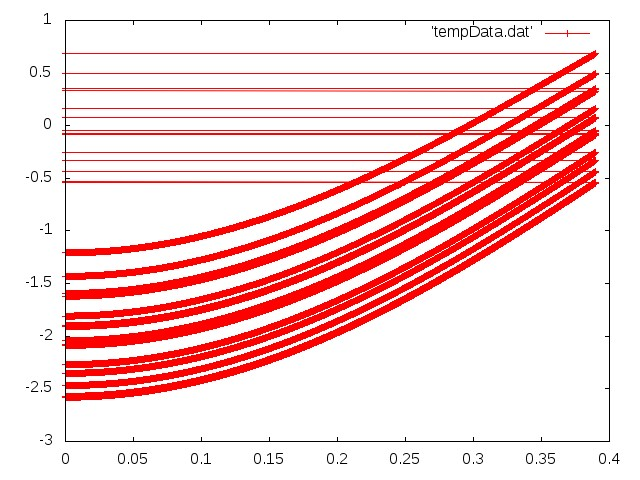
\includegraphics[width=0.3\columnwidth]{Chapter2/Figs/Raster/harmonic1.jpeg}}~~~\subfloat{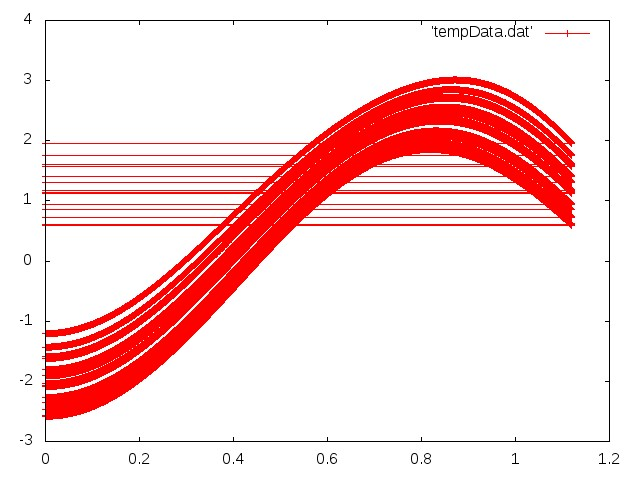
\includegraphics[width=0.3\columnwidth]{Chapter2/Figs/Raster/harmonic2.jpeg}}~~~\subfloat{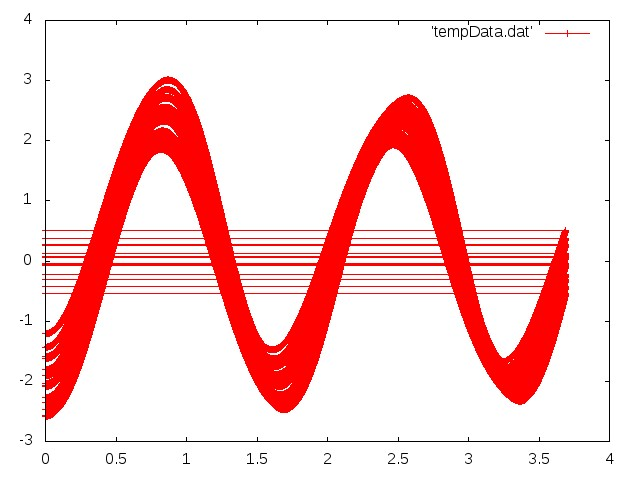
\includegraphics[width=0.3\columnwidth]{Chapter2/Figs/Raster/harmonic.jpeg}}
\par\end{centering}

\caption{Simulated Bohmian trajectories for a harmonic oscillator.\label{fig:Simulated-Bohmian-Trajectories}}


\selectlanguage{english}%
\selectlanguage{english}%
\end{figure}



\subsection{Simulation Results\label{sub:BM-Simulation-Results}}

BM was successfully simulated for a particle, with a single degree
of freedom, influenced by an arbitrary potential. Implementing RK4,
interpolation and random distribution generation were among the non-trivial
aspects. Generalization to multiple particles and inclusion of spins,
was among the immediate next steps, however due to later theoretical
developments, were not carried out. The code is available at \cite{gitHubThesisSim}
%\href{https://github.com/toAtulArora/msThesis/tree/master/numerics}{github.com/toAtulArora/msThesis/tree/master/numerics}.


\section{Measurements in BM (I)\label{sec:Measurements-in-BM}}

Measurement of spins in BM was discussed in the previous chapter.
Our interest in this chapter, is in measuring $q$, $p$ and functions
there of. We will learn that one can infact construct a universal
method that facilitates the measurement of any arbitrary observable.
The analysis will clarify two notions which are at high risk of being
misconstrued. First, that the position of the particle, when measured,
will infact yield $q$. However, a measurement of momentum of a particle,
as we will see, does not always yield $p$ (the value it had prior
to measurement). Infact, it would be inconsistent with QM if it did;
for instance, consider $\psi(q)=\left(1/\sqrt{\pi}\right)e^{-q^{2}}$,
for which $S=0$ and therefore so is $p=\nabla S=0$. However it is
known that upon measurement of momentum, one obtains a distribution
given by the fourier transform of $\psi$. Although this is centred
around the origin, it is not a delta function (has non-zero spread).
The second notion which is clarified, is that to find the value obtained
upon measurement of certain observables, knowledge about the precise
position of the measuring particle (the particle used to make the
measurement) can play a deciding role.


\subsection{Observable with discrete spectrum | Hamiltonian Approach}

Bohm has discussed in his second paper \cite{Bohm2}, how any arbitrary
observable maybe measured, in BM. To describe a measurement, we use
a measuring particle (mass $m_{L}$, say), by getting it to interact
with the system for a short duration appropriately. Subsequently,
we measure the final position of the particle, to learn about the
value of the observable of interest. Say for instance, we wish to
measure the observable $\hat{L}$, then the required interaction Hamiltonian
is given by $\hat{H}_{\text{int}}=a\hat{L}\otimes\hat{p}$. Here the
first operator acts on the system and second (after the tensor product
symbol) acts on the measuring particle. $a$ quantifies the interaction
strength. It has dimensions of frequency, if $L$ has dimensions of
length. Let us assume that the system in the state $\left|\psi\right\rangle $.
Then it is known that one can express $\left|\psi\right\rangle =\sum_{l}\left\langle l|\psi\right\rangle \left|l\right\rangle $,
where $\left|l\right\rangle $ are the eigenstates of $\hat{L}$ with
eigenvalue $l$ (we have assumed non-degenercy for simplicity, but
its removal doesn't cause any significant difficulty). $\left|\Psi_{S}(t)\right\rangle =\hat{U}(t)\left|\psi\right\rangle \otimes\left|\varphi\right\rangle $,
where 
\[
\hat{U}(t)=e^{-\frac{i}{\hbar}\left[-\hbar^{2}\frac{\nabla_{1}^{2}}{2m}-\hbar^{2}\frac{\nabla_{2}^{2}}{2m_{L}}+\hat{H}_{\text{int}}\right]t}
\]
 and $\left|\varphi\right\rangle $ is the state of the measuring
particle, given by a Guassian centred at the origin, $\varphi(q)=(1/\sqrt{2\pi}\sigma)e^{-q^{2}/2\sigma^{2}}$.
If $t$ is very small, and $a$ very large, s.t. $at=\lambda$ is
a finite number, then one can neglect the free evolution, $\nabla^{2}t$
terms compared to $\hat{H}_{\text{int}}t$. We then have 
\begin{eqnarray*}
\left|\Psi_{S}(t)\right\rangle  & = & e^{-\frac{i}{\hbar}a\hat{L}\otimes\hat{p}t}\left|\Psi_{S}\right\rangle \\
 & = & \sum_{l}\left\langle l|\psi\right\rangle \left|l\right\rangle \otimes e^{-\frac{i}{\hbar}\lambda l\,\hat{p}}\left|\varphi\right\rangle \\
 & = & \sum_{l}\left\langle l|\psi\right\rangle \left|l\right\rangle \otimes\left|\varphi_{\lambda l}\right\rangle ,
\end{eqnarray*}
where $\left|\varphi_{q_{0}}\right\rangle =\int dq\varphi(q-q_{0})\left|q\right\rangle $.
This interaction, effectively entangles the measuring particle, with
the possible `outcomes', eigenstates of the observable $\hat{L}$
of interest. If $\sigma\ll\lambda l$, then according to QM itself,
a position measurement of the measuring particle, would correspond,
in a one-to-one way, to the eigenstate/eigenvalue of $\hat{L}$, to
which the system will collapse. In the context of BM, after the interaction,
the measuring particle would be guided into one of these eigenstates,
and a position measurement would yield the same. We glossed over various
details in making the last statement, which will be delineated shortly,
through some illustrations. 


\subsubsection{Generalization to observables with continuum spectrum \label{sub:BM-measurement-to-continuous}}

Since we are interested in observing phase space variables, the aforesaid
must be generalized to the continuous spectrum regime. We proceed
with the aforesaid notation, and promote the discrete operator $\hat{L}$
to have a continuous spectrum. Thus $\left|\psi\right\rangle =\int dl\left\langle l|\psi\right\rangle \left|l\right\rangle $,
and recall $\left|\varphi\right\rangle =\int dq\varphi(q)\left|q\right\rangle $,
where $\varphi(q)$ has $\sigma$ quantifying the deviation from the
origin. Now $\left|\Psi_{S}(t)\right\rangle =\hat{U}(t)\left|\psi\right\rangle \otimes\left|\varphi\right\rangle =\int\int dldq\varphi(q)\left\langle l|\psi\right\rangle \left|l\right\rangle \otimes\left|q+l\lambda\right\rangle $,
where $\lambda=at$ as before. Say $q$ is measured at this stage
and $q'$ is the value obtained. The resultant state would then be
$\left|q'\right\rangle \left\langle q'\right|\left|\Psi_{S}\right\rangle =\int\int dldq\varphi(q-l\lambda)\left\langle l|\psi\right\rangle \left|l\right\rangle \delta(q-q')=\int dl\varphi(q'-l\lambda)\left\langle l|\psi\right\rangle \left|l\right\rangle $.
We know that $\varphi(q)\approx0$ when $q\notin(-\delta q,\delta q)$,
where $\delta q=\mathcal{O}(\sigma)$ can be chosen, depending on
the accuracy desired. This implies $-\delta q<q'-l\lambda<\delta q$,
which entails that $l=\frac{q'}{\lambda}\pm\frac{\delta q}{\lambda}$.
We thus have a relation between the observed position, $q'$, of the
measuring particle, and the value of the operator $\hat{L}$. The
error is controlled by the sharpness of the initial state of the measuring
particle.


\subsubsection{Consistency check; measurement of position \label{sub:BM-Consistency-check-measurement}}

The position of a particle, as is claimed by BM, remains the same
upon observing. Let us verify this statement, by applying the aforesaid
formalism. For simplicity, let us assume that the state of the system
is given as $\sqrt{2}\left|\psi\right\rangle =\int dq\left[\delta(q-q_{0})+\delta(q+q_{0})\right]\left|q\right\rangle $,
which is to say, the system is in a superposition of being at $q_{0}$
and $-q_{0}$. Let us assume that the particle is initially given
to be in $q_{1}=q_{0}$. Now our measurement formalism must be consistent
with this, viz. the answer must not depend on the initial position
of the measuring particle. Initially then, the state is $\left|\Psi_{S}\right\rangle =\left|\psi\right\rangle \otimes\left|\varphi\right\rangle $,
while after interaction, the state becomes $\sqrt{2}\left|\Psi_{S}(t)\right\rangle =\left|q_{0}\right\rangle \otimes\left|\varphi_{\lambda q_{0}}\right\rangle +\left|-q_{0}\right\rangle \otimes\left|\varphi_{-\lambda q_{0}}\right\rangle $.
To understand this clearly, one must plot $\left|\Psi_{S}(q_{1},q_{2})\right|^{2}=\left|\left\langle q_{1},q_{2}|\Psi_{S}\right\rangle \right|^{2}$,
where $\left|q_{1}\right\rangle $ is (the position eigenket) for
the system and $\left|q_{2}\right\rangle $ for the measuring particle.
\begin{figure}
\begin{centering}
\subfloat[Before interaction\label{fig:PosMes-Before-interaction}]{\begin{centering}
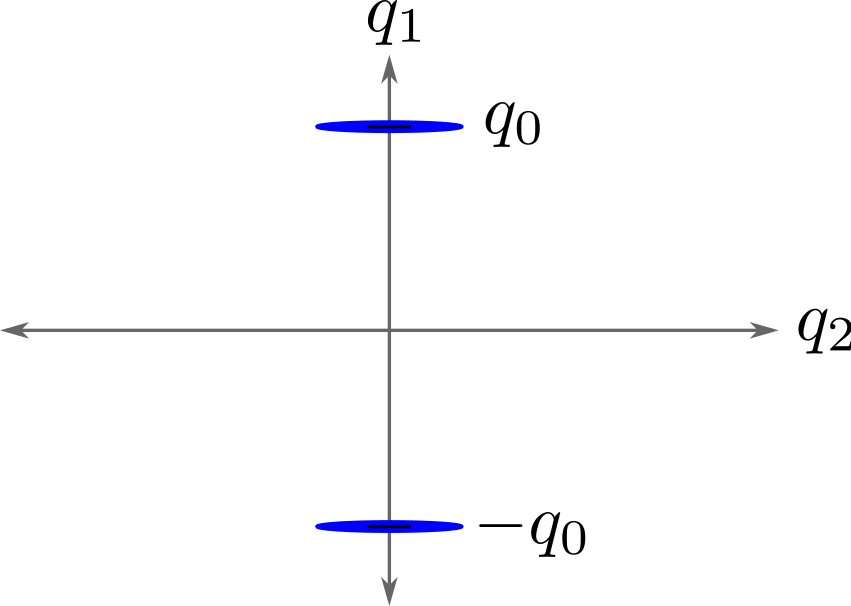
\includegraphics[width=0.45\textwidth]{Chapter2/Figs/Raster/posMesBefore}
\par\end{centering}

\selectlanguage{english}%
\selectlanguage{english}%
}~~ ~~\subfloat[After interaction\label{fig:PosMes-After-interaction}]{\begin{centering}
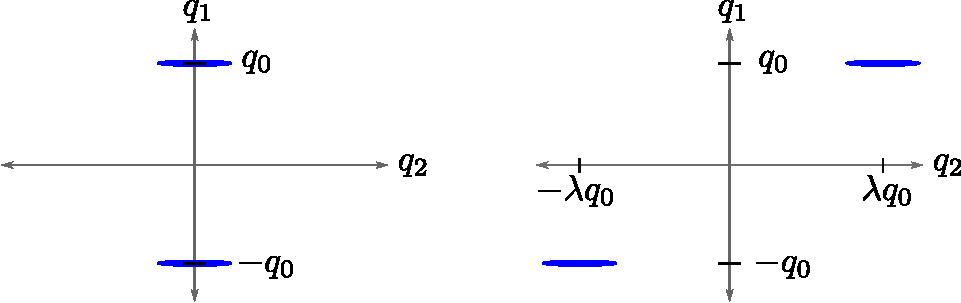
\includegraphics[width=0.45\textwidth]{Chapter2/Figs/Raster/posMesAfter}
\par\end{centering}



\selectlanguage{english}%
\selectlanguage{english}%
}
\par\end{centering}

\caption{Indicative contour plot of $\left|\left\langle q_{1},q_{2}|\Psi_{S}\right\rangle \right|^{2}$,
illustrating consistency of position measurements. }


\selectlanguage{english}%
\selectlanguage{english}%
\end{figure}
Before the interaction (see \prettyref{fig:PosMes-Before-interaction}),
say the measuring particle was at $q_{2}\in(-\sigma,\sigma)$. After
the interaction (see \prettyref{fig:PosMes-After-interaction}), the
measuring particle will move to $q_{2}\in(\lambda q_{0}-\sigma,\lambda q_{0}+\sigma)$,
which follows simply by noting that the velocities are given by probability
current. A measurement of the particle's position would yield $q_{2}\approx\lambda q_{0}$,
which we know from our analysis, corresponds to $q_{1}=q_{0}$, which
is infact consistent with our initial conditions. It must be emphasized
that the position of the measuring particle, plays no essential role
in deciding where it would show up. The same analysis can be repeated
for $q_{1}=-q_{0}$ and in this case, from \prettyref{fig:PosMes-After-interaction},
it would follow that after the interaction, $q_{2}\approx-\lambda q_{0}$.
Consistency of this method is therefore established. Ofcourse, one
can relax the idealized $\delta$ functions to obtain more realistic
functions, but the conclusion remains invariant.


\subsubsection{Consistency check; measurement of momentum}

We now resolve the issue pointed out in the beginning of this section,
viz. the observed value of $p$ being inconsistent with QM. We begin
with writing the state of the system as $\left|\psi\right\rangle =\int dq\left(1/\sqrt{\pi}\right)e^{-q^{2}}\left|q\right\rangle $,
so that $p=\nabla S=0$. We wish to find, how the spread in the observed
value of $p$ appears, from the aforesaid measurement formalism. Note
that 
\begin{eqnarray*}
\left|\psi\right\rangle  & = & \int dp\left|p\right\rangle \int dq\cancelto{\left(1/\sqrt{2\pi\hbar}\right)e^{-iqp/\hbar}}{\left\langle p|q\right\rangle }\psi(q)\\
 & = & \int dp\tilde{\psi}(p)\left|p\right\rangle ,
\end{eqnarray*}
where $\tilde{\psi}(p)$ is $\psi(q)$ fourier transformed. The combined
state before measurement is given by $\left|\Psi_{S}\right\rangle =\left|\psi\right\rangle \otimes\left|\varphi\right\rangle $,
while after the measurement, $\left|\Psi(t)\right\rangle =\int dp\tilde{\psi}(p)\left|p\right\rangle \otimes\left|\varphi_{\lambda p}\right\rangle $.
The aforesaid expression entails that, assuming $\sigma\to0$, the
probability for the measuring particle, to end up at $\lambda p$,
is given by $\left|\tilde{\psi}(p)\right|^{2}$, which is consistent
with QM. To obtain this result more carefully from Bohmian trajectories,
one must plot $\left|\left\langle q_{1},q_{2}|\Psi_{S}\right\rangle \right|^{2}$
as was done in the previous section, but we will satisfy ourselves
here, with noting that the measurement process has explicitly imparted
momentum on the system, as is clear after `collapsing' the wavefunction.


\subsection{Classical limit of measurements}

Although we have not yet discussed the classical limit of BM, as an
aside, it maybe demonstrated that this indeed follows elegantly. If
we write $\psi=Re^{iS/\hbar}$ and substitute this in the Schr\"odinger
Equation, and separate the real and imaginary parts, we obtain 
\begin{eqnarray*}
\frac{\partial R}{\partial t} & = & -\frac{1}{2m}\left[R\nabla^{2}S+2\nabla R.\nabla S\right],\\
\frac{\partial S}{\partial t} & = & -\left[\frac{\nabla S^{2}}{2m}+V-\frac{\hbar^{2}}{2m}\frac{\nabla^{2}R}{R}\right].
\end{eqnarray*}
The reader would've recognized that the second equation is essentially
the Hamilton Jacobi equation, with an extra term. Infact, if one writes
$P=R^{2}$, then we obtain 
\begin{eqnarray*}
\frac{\partial P}{\partial t}+\nabla.\left(P\frac{\nabla S}{m}\right) & = & 0\\
\frac{\partial S}{\partial t}+\frac{\nabla S^{2}}{2m}+V-\frac{\hbar^{2}}{4m}\left[\frac{\nabla^{2}P}{P}-\frac{1}{2}\frac{\nabla P^{2}}{P^{2}}\right] & = & 0
\end{eqnarray*}
which makes the first equation effectively a continuity equation for
probabilities, if one relates $\nabla S=p$ (momentum in BM), as is
done in the Hamilton Jacobi framework. Effectively then, BM elegantly
yields the classical limit, for if we neglect the $\hbar$ term, then
we have particles obeying Newton's laws. 

Our motivation was to study how the measured value of momentum turns
out to be $p=\nabla S$ in the classical limit. The larger goal, was
to use this elegant framework, to understand how measurement of functions
of $q,\,p$, such as the energy for example, become equivalent to
measuring $q$ and $p$ and plugging their values into the function.
To be precise, consider the example of an energy eigenstate in a harmonic
potential. For this state, neither $q$ nor $p$ are precisely defined
(in the language of QM), however, the energy is sharp. We started
with analysing the classical limit of the measurement process, just
discussed. That requires the potential $V$, to be a function of both
$q$ and $p$, whereas for the aforesaid derivation, only position
dependent $V$ was used. Correcting for this, create various issues.
First of all, this interaction adds a term to the continuity equation,
\[
\frac{\partial P}{\partial t}+\nabla_{1}\left(P\frac{\nabla_{1}S}{m}\right)+\nabla_{2}\left(P\frac{\nabla_{2}S}{m}\right)+\overbrace{2aR\left[\nabla_{1}R\nabla_{2}S+R\nabla_{1}\nabla_{2}S+\nabla_{2}R\nabla_{1}S\right]}^{\text{Extra Term! | How will}\,P\,\text{satisfy the continuity equation?}}=0.
\]
The interaction also adds a ``quantum potential'' in addition to the
expected potential, which doesn't seem to disappear in the large mass
limit, 
\[
\frac{\partial S}{\partial t}+\frac{(\nabla_{1}S)^{2}}{2m}+\frac{(\nabla_{2}S)^{2}}{2m}+\overbrace{a\nabla_{1}S\nabla_{2}S}^{\text{expected part}}-\overbrace{a\hbar^{2}\frac{\nabla_{1}\nabla_{2}R}{R}}^{\text{\text{quantum part}}}-\underbrace{\frac{\hbar}{2mR}(\nabla_{1}^{2}R+\nabla_{2}^{2}R)}_{\text{usual quantum potential}}=0.
\]
One can see that with $\hbar\to0$, the quantum potential and the
quantum part of the interaction, both disappear. However, the continuity
equation is not recovered still. This part was not explored further,
but can perhaps be studied independent of our current target.


\subsection{Measurement Exploration Summarized}

From the optimized GHZ construction, it was necessary to arrive at
a theoretical construction, that would allow calculation of measurement
outcomes associated with arbitrary operators composed using $\hat{q},\,\hat{p}$.
This was achieved, however it was found that obtaining these results
is not trivial in most cases of interest. The surprising result, that
measurement of $\hat{p}$ may not yield $p=\nabla S$, while a measurement
of $\hat{q}$ yields $q$, was derived and clarified. This takes us
a step closer to understanding how BM can explain the optimized (or
even the phase space) GHZ test, by allowing an in principle simulation.


\section{Roy Singh Theory }

Roy Singh (RS) proposed \cite{roySingh} a causal completion of QM,
that treated position and momentum symmetrically. In their theory,
the joint probability distribution was such that when the momentum
is integrated out, the result agrees with quantum mechanical predictions
for position \emph{and} when positions are integrated out, they agree
with the quantum mechanical momentum distribution. This was rather
interesting for, BM fails to do the latter, and requires more analysis
to resolve (as was discussed in the previous section). This joint
probability distribution, given by RS, could indeed be thought of
as describing the phase space of real particles, for it was positive
everywhere, unlike the Wigner distribution. The cost however was that
evaluation of arbitrary functions of $q,p$ was not as simple as integrating
it over the joint distribution. While a promising framework and interesting
in its own right, in the light of the optimized GHZ test, it wasn't
particularly helpful. It was not pursued beyond a preliminary reading
stage. 


\section{Remarks}

In summary then, we have looked at a version of the GHZ test, the
phase space extension. This effectively says that $\hat{q},\hat{p}$
can't have pre-defined values. Now, even though BM has pre-defined
values for $q,p$ in principle, upon measurement, we learnt that the
value of $p$ can change. Infact, it may very well depend on the initial
position of the measuring particle. To be able to test this quantitatively,
we had to (a) optimize the phase space GHZ test, (b) learn more about
measurements and (c) write an appropriate BM simulator. Progress was
made on each front and the results discussed. However, the crucial
point is that even in BM, the measurements correspond to operators.
It entails therefore that measuring $ABC\neq D$ but infact\footnote{where $A,B,C,D$ are as defined for the spin GHZ, and the argument
essentially holds even for the phase-space (optimized) GHZ} $ABC=-D$, even from the point of view of BM, a deterministic theory.
This hinges essentially on whether we can commute the operators that
were used to construct $A,B$ and $C$ to start with, which even in
BM we can't. Stated another way, we learn that $YXY\neq Y^{2}X=X$,
but $YXY=-Y^{2}X=-X$, even in BM, where these operators have pre-defined
values (given all initial conditions). This is simply because $X$
and $Y$ are operators and they anti-commute. So even though numerically
we haven't quite proven that BM will be consistent, qualitative cogent
arguments already suggest that BM will infact turn out to be consistent
with QM. What will remain, will be a matter of detail.

\begin{comment}

\section{My First Section}

I'm going to randomly include a picture Figure. If you have trouble
viewing this document contact Krishna: \href{mailto:kks32@cam.ac.uk}{kks32@cam.ac.uk}


\subsection{Enumeration }
\begin{enumerate}
\item The first topic is dull
\item The second topic is duller 

\begin{enumerate}
\item The first subtopic is silly 
\item The second subtopic is stupid 
\end{enumerate}
\item The third topic is dullest
\end{enumerate}

\subsection{Itemized}
\begin{itemize}
\item The first topic is dull
\item The second topic is duller 

\begin{itemize}
\item The first subtopic is silly 
\item The second subtopic is stupid 
\end{itemize}
\item The third topic is dullest
\end{itemize}

\section{My Second Section}

Lorem ipsum dolor sit amet, consectetur adipiscing elit. In magna
nisi, aliquam id blandit id, congue ac est. Fusce porta consequat
leo. Proin feugiat at felis vel consectetur. Ut tempus ipsum sit amet
congue posuere. Nulla varius rutrum quam. Donec sed purus luctus,
faucibus velit id, ultrices sapien. Cras diam purus, tincidunt eget
tristique ut, egestas quis nulla. Curabitur vel iaculis lectus. Nunc
nulla urna, ultrices et eleifend in, accumsan ut erat. In ut ante
leo. Aenean a lacinia nisl, sit amet ullamcorper dolor. Maecenas blandit,
tortor ut scelerisque congue, velit diam volutpat metus, sed vestibulum
eros justo ut nulla. Etiam nec ipsum non enim luctus porta in in massa.
Cras arcu urna, malesuada ut tellus ut, pellentesque mollis risus.Morbi
vel tortor imperdiet arcu auctor mattis sit amet eu nisi. Nulla gravida
urna vel nisl egestas varius. Aliquam posuere ante quis malesuada
dignissim. Mauris ultrices tristique eros, a dignissim nisl iaculis
nec. Praesent dapibus tincidunt mauris nec tempor. Curabitur et consequat
nisi. Quisque viverra egestas risus, ut sodales enim blandit at. Mauris
quis odio nulla. Cras euismod turpis magna, in facilisis diam congue
non. Mauris faucibus nisl a orci dictum, et tempus mi cursus. Etiam
elementum tristique lacus, sit amet eleifend nibh eleifend sed 1 .
Maecenas dapibu augue ut urna malesuada, non tempor nibh mollis. Donec
sed sem sollicitudin, convallis velit aliquam, tincidunt diam. In
eu venenatis lorem. Aliquam non augue porttitor tellus faucibus porta
et nec ante. Proin sodales, libero vitae commodo sodales, dolor nisi
cursus magna, non tincidunt ipsum nibh eget purus. Nam rutrum tincidunt
arcu, tincidunt vulputate mi sagittis id. Proin et nisi nec orci tincidunt
auctor et porta elit. Praesent eu dolor ac magna cursus euismod. Integer
non dictum nunc.

\begin{figure}
\hfill{}
\includegraphics[width=0.3\textwidth,bb = 0 0 200 100, draft, type=eps]{Chapter2/Figs/Raster/minion.png}\hfill{}

\caption{Minions from Despicable Me}
\end{figure}


% Begin Landscape Layout
\begin{landscape}

\begin{figure}
\subfloat[Minions]{\begin{centering}

\includegraphics[width=0.3\columnwidth,bb = 0 0 200 100, draft, type=eps]{Chapter2/Figs/Raster/minion.png}
\par\end{centering}

}\subfloat[Tom and Jerry]{\begin{centering}

\includegraphics[width=0.3\columnwidth,bb = 0 0 200 100, draft, type=eps]{Chapter2/Figs/Raster/TomandJerry.png}
\par\end{centering}

}\subfloat[Wall-E]{\begin{centering}
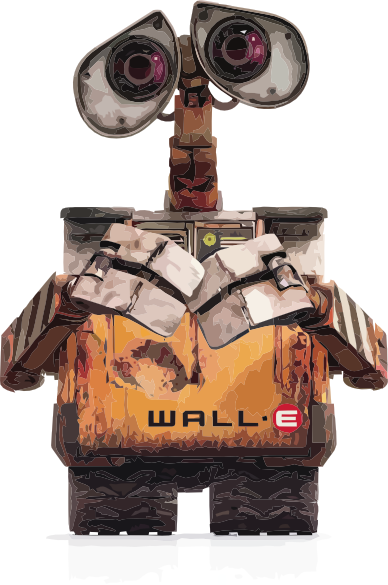
\includegraphics[width=0.3\columnwidth,bb = 0 0 200 100, draft, type=eps]{Chapter2/Figs/Raster/WallE.png}
\par\end{centering}

}

\caption{Best Animation Movies}
\end{figure}


% End Landscape Layout
\end{landscape}
\end{comment}
\selectlanguage{english}%



\selectlanguage{british}%

\chapter{Contextuality and Bohmian Mechanics}


\section{Rationale}

We saw in the last chapter that BM is able to explain the GHZ test.
The paradox arises if we try to multiply values assigned to operators
that don't commute, to obtain the value assigned to a product of such
operators. In BM, since the operator must be provided to obtain it's
value, no contradiction arises, even though the results are deterministic
(given all initial conditions). %
\begin{comment}
Effectively then, at the risk of repetition, the flaw in our GHZ reasoning,
was that we were commuting operators that didn't commute, by assuming
they were numbers.
\end{comment}
Thus, we were only able to rule out theories that treated operators
like numbers and we find that BM is not one of them. However, as we
have seen in the Peres Mermin (PM) test, the operators whose values
are multiplied, do infact commute, implying that the PM test is exonerated
from that objection. And we also know that BM, atleast on the face
of it, is non-contextual, viz. the value obtained upon the measurement
of an operator, depends only on the state (+ hidden variables) and
the operator, granted we fix our measurement scheme. It is therefore
not clear how BM is contextual, which is a notion we're forced to
accept from the PM test. Further, since BM is claimed to reproduce
all results of QM, does it entail that a non-contextual theory can
explain the PM test?

We also found in the previous chapter, that in BM, there's no fundamental
difference that arises between the phase space variables and spins.
As we saw, the value of momentum observed, depends on the systematics
of the measurement process, just as the outcome of a spin measurement
using an SG setup (as was discussed in the first chapter). Therefore
in what follows, attempts will be made at tackling the problem from
whichever method, (between phase space and spins) appears more accessible. 


\section{Intensifying Contextuality}

We have already seen that GHZ test is a test of determinism, of whether
predefined values can explain QM, while the PM test is that of contextuality,
which says that predefined non-contextual values, a more subtle remark,
can't explain QM. We also learnt how one can extend the GHZ test to
continuous variables. In this section, we will make both these schemes
effectively equally powerful; make GHZ into a test of contextuality
and extend the PM test to continuous variables. 


\subsection{GHZ escalated to Contextuality \label{sub:GHZ-to-contextuality}}

Recall from the first chapter, $\hat{A}\equiv\sigma_{x}\otimes\sigma_{y}\otimes\sigma_{y}$,
$\hat{B}\equiv\hat{\sigma}_{y}\otimes\hat{\sigma}_{x}\otimes\hat{\sigma}_{y}$,
$\hat{C}\equiv\hat{\sigma}_{y}\otimes\hat{\sigma}_{y}\otimes\hat{\sigma}_{x}$
and $\hat{D}=\hat{\sigma}_{x}\otimes\hat{\sigma}_{x}\otimes\hat{\sigma}_{x}$,
and $\hat{A}\hat{B}\hat{C}=-\hat{D}$. Consider now, in addition,
the following operators, 
\[
\hat{H}_{ij}\doteq\left[\begin{array}{ccc}
\hat{\sigma}_{x}\otimes\hat{\mathbb{I}}\otimes\hat{\mathbb{I}}^{(a)} & \hat{\mathbb{I}}\otimes\hat{\sigma}_{y}\otimes\hat{\mathbb{I}}^{(2)} & \mathbb{\hat{I}}\otimes\mathbb{\hat{I}}\otimes\hat{\sigma}_{y}^{(3)}\\
\hat{\sigma}_{y}\otimes\mathbb{\hat{I}}\otimes\hat{\mathbb{I}}^{(1)} & \hat{\mathbb{I}}\otimes\hat{\sigma}_{x}\otimes\hat{\mathbb{I}}^{(b)} & \mathbb{\hat{I}}\otimes\hat{\mathbb{I}}\otimes\hat{\sigma}_{y}^{(3)}\\
\hat{\sigma}_{y}\otimes\mathbb{\hat{I}}\otimes\hat{\mathbb{I}}^{(1)} & \mathbb{\hat{I}}\otimes\hat{\sigma}_{y}\otimes\hat{\mathbb{I}}^{(2)} & \mathbb{\hat{I}}\otimes\hat{\mathbb{I}}\otimes\hat{\sigma}_{x}^{(c)}\\
\hat{\sigma}_{x}\otimes\mathbb{\hat{I}}\otimes\hat{\mathbb{I}}^{(a)} & \mathbb{\hat{I}}\otimes\hat{\sigma}_{x}\otimes\hat{\mathbb{I}}^{(b)} & \hat{\mathbb{I}}\otimes\hat{\mathbb{I}}\otimes\hat{\sigma}_{x}^{(c)}
\end{array}\right]
\]
and note that (a) the product of these operators along each row, yields
$\hat{A}$, $\hat{B}$, $\hat{C}$ and $\hat{D}$ respectively, (b)
operators along any row, commute and (c) the superscript labels identify
operators that are repeated. 

We will now try to assign values to $\hat{H}_{ij}$ and only multiply
values assigned to commuting observables, to obtain the value of $\hat{A},\hat{B},\hat{C}$
and $\hat{D}$. We know (see \prettyref{sec:Determinism-The-GHZ})
that according to QM, for the GHZ state, $\left|\chi_{G}\right\rangle $,
$\hat{A},\,\hat{B}$ and $\hat{C}$ must be assigned the value $+1$,
while $\hat{D}$ must be assigned $-1$. We demand that our assignment
corresponds to this state. Let us start with assigning values to the
last row. To obtain a $-1$ corresponding to $D$, we must have either
a $1,1,-1$ (or permutations) or $(-1,-1,-1)$. Let us assume that
the former is true. At this stage then, we'd have 
\[
H_{ij}\doteq\left[\begin{array}{ccc}
1\\
 & 1\\
 &  & -1\\
1 & 1 & -1
\end{array}\right].
\]
Now to obtain a $+1$ in the first row (for $A$), we must have $(1,\pm1,\pm1)$.
Similarly we get, for the second row, $(\pm1,1,\pm1)$. The assignment
then becomes 
\[
H_{ij}\doteq\left[\begin{array}{ccc}
1 & \pm1 & \pm1\\
\pm1 & 1 & \pm1\\
\pm1 & \pm1 & -1\\
1 & 1 & -1
\end{array}\right],
\]
however, we have no freedom left and are forced to assign $-1$ to
the third row, while we were required to have it equal $+1$. A little
reflection reveals that the $(-1,-1,-1)$ case for the last row, won't
resolve the issue. Thus we conclude that the assignment must be contextual
(atleast the one corresponding to $\left|\chi_{G}\right\rangle $).
In this scenario, the non-commuting observables argument, deduced
in the previous chapter fails. Here, values of only commuting observables
were multiplied, even though effectively it is still the same GHZ
test.


\subsection{Peres Mermin escalated to Continuous Variables \label{sub:Peres-Mermin-phaseSpace}}

The Peres Mermin situation can be, quite simply, extended to continuous
variables, which maybe of practical interest. Performing SG type setup
in the simulation requires implementation of spins and appropriate
magnetic field effects, and that can be surpassed with this construction.
To this end, the following extension was worked out (but this result
was already known \cite{contextualityPhaseSpace}). For any unitary
operators $\hat{X}$ and $\hat{Y}$, s.t. $\{\hat{X},\hat{Y}\}=0$
and so is $\{\hat{X},\hat{Y}^{\dagger}\}=0$, if we define $\hat{Z}=i\hat{Y}\hat{X}$,
then 
\[
\begin{array}{ccc}
\hat{X}\otimes\hat{\mathbb{I}} & \hat{\mathbb{I}}\otimes\hat{X} & \hat{X}^{\dagger}\otimes\hat{X}^{\dagger}\\
\hat{\mathbb{I}}\otimes\hat{Y} & \hat{Y}\otimes\hat{\mathbb{I}} & \hat{Y}^{\dagger}\otimes\hat{Y}^{\dagger}\\
\hat{X}^{\dagger}\otimes\hat{Y}^{\dagger} & \hat{Y}^{\dagger}\otimes\hat{X}^{\dagger} & \hat{Z}\otimes\hat{Z}
\end{array}
\]
would yield the PM situation. To check this, note that the product
along any row, is $\hat{\mathbb{I}}$ and it is also so for each column,
except for the third, which is $-\hat{\mathbb{I}}$, precisely the
same as the PM situation. The difference however, will be that the
corresponding hidden variables, will have to be unimodular complex
(viz. $XX^{*}=1$) and the values of the operators, must be deduced
from their hermitian counterparts. One such choice of $X$ and $Y$
was pointed out in the previous chapter; $\hat{X}\equiv e^{i\sqrt{\pi}\hat{q}/\hbar L}$
and $\hat{Y}\equiv e^{i\sqrt{\pi}\hat{p}L/\hbar}$. Note that in this
case, optimization is not required, for this test is state independent
(should work with any choice of states).


\section{Measurements in BM (II)}

Measurements have already been discussed at length in the previous
chapters, however, we are now particularly interested in measuring
spins, especially when there is entanglement. We will see how a measurement
made using the Stern Gerlach like apparatus can yield results very
different from those obtained by the Hamiltonian approach. Further,
we will see how the former can get difficult to evaluate, quite quickly.


\subsection{Stern Gerlach based measurements \label{sub:BM-entangled-Stern-Gerlach}}

Since we have already discussed how to analyse a Stern Gerlach based
measurement for a single particle, let us try to explore how to analyse
this for $\left|\chi\right\rangle =\left|++\right\rangle +\left|--\right\rangle /\sqrt{2}$,
where for instance $\left|++\right\rangle =\left|+\right\rangle _{A}\otimes\left|+\right\rangle _{B}$
($A$ and $B$ label the particle), and $\hat{\sigma}_{x}\otimes\hat{\sigma}_{x}$
is the observable of interest. Borrowing the notation and the analysis
from \prettyref{sec:Bohm's-Theory,-Bohmian}, we have $\sqrt{2}\left|\Psi_{S}\right\rangle =\left|\psi,\psi\right\rangle \otimes\left[\left|++\right\rangle +\left|--\right\rangle \right]$
initially and after the interaction, $\sqrt{2}\left|\Psi_{S}(t)\right\rangle =\left|\psi_{at},\psi_{at}\right\rangle \otimes\left|++\right\rangle +\left|\psi_{-at},\psi_{-at}\right\rangle \otimes\left|--\right\rangle $,
where $\left|\psi_{at},\psi_{at}\right\rangle =\left|\psi_{at}\right\rangle _{A}\otimes\left|\psi_{at}\right\rangle _{B}$
for example. Now, we must predict the outcome, given the initial positions
of the particles. We then plot $P(q_{1},q_{2})=\left\langle \Psi_{S}|q_{1},q_{2}\right\rangle \left\langle q_{1},q_{2}|\Psi_{S}\right\rangle $,
where $q_{1}$ and $q_{2}$ represent the $z$ coordinate of the particles,
and effectively we are summing over the spin degree of freedom, asking
for the probability of finding the particles near $q_{1}$ and $q_{2}$.
Initially, $P=\left|\left\langle q_{1},q_{2}|\psi,\psi\right\rangle \right|^{2}$
which would yield circles in a contour plot (showing say 70\% probability
enclosed within), see \prettyref{fig:sgMeas-Initial-State}. 
\begin{figure}
\begin{centering}
\subfloat[Initial State \label{fig:sgMeas-Initial-State}]{\begin{centering}
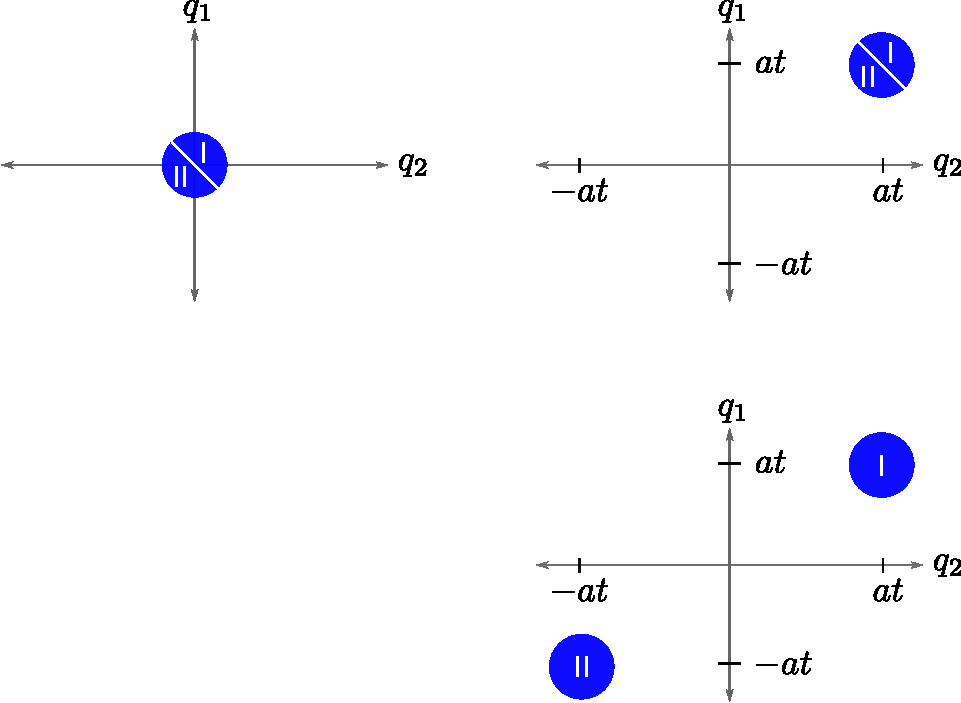
\includegraphics[width=0.3\columnwidth]{Chapter3/Figs/Raster/initial}
\par\end{centering}



\selectlanguage{english}%
\selectlanguage{english}%
}\subfloat[For $\sqrt{2}\left|\chi\right\rangle =\left|00\right\rangle +\left|11\right\rangle $\label{fig:sgMeas-Entangled}]{\begin{centering}
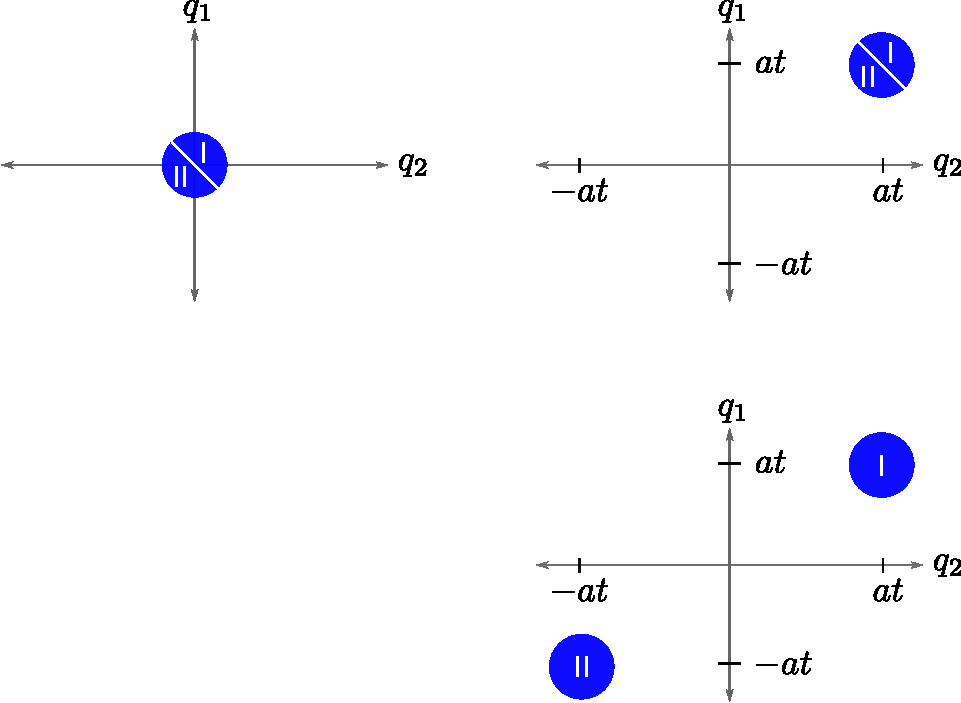
\includegraphics[width=0.3\columnwidth]{Chapter3/Figs/Raster/finalEntangled}
\par\end{centering}



\selectlanguage{english}%
\selectlanguage{english}%
}\subfloat[For $\left|\chi\right\rangle =\left|++\right\rangle $\label{fig:sgMeas-++}]{\begin{centering}
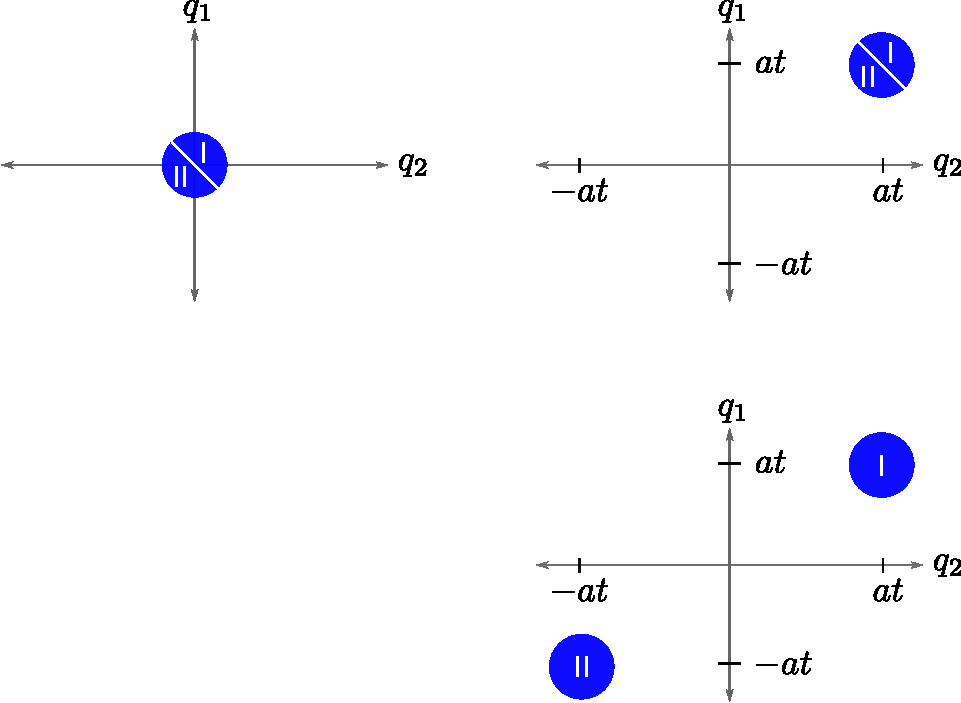
\includegraphics[width=0.3\columnwidth]{Chapter3/Figs/Raster/final}
\par\end{centering}

}
\par\end{centering}

\caption{Indicative contour plots for $\left|\left\langle q_{1},q_{2}|\Psi_{S}\right\rangle \right|^{2}$,
illustrating spin measurement of 2 particles, using the Stern Gerlach
setup.}


\selectlanguage{english}%
\selectlanguage{english}%
\end{figure}
After the interaction, $2P(q_{1},q_{2})=\left|\left\langle q_{1},q_{2}|\psi_{at},\psi_{at}\right\rangle \right|^{2}+\left|\left\langle q_{1},q_{2}|\psi_{-at},\psi_{-at}\right\rangle \right|^{2}$,
which would yield two circles in the countour plot, one centred at
$(at,at)$ and the other centred at $(-at,-at)$, see \prettyref{fig:sgMeas-Entangled}.
From the symmetry of the problem, and from the fact that velocities
are single valued, we can deduce that if the particle positions were
represented by a point inside area $I$, then the result would be
a spin up, viz. $\left|+\right\rangle $ for both, while for the other
case, the result would be spin down for both. Note that there's no
initial condition for which the results are anti-correlated, consistent
with $\left|\chi\right\rangle $. Although it is obvious, it is instructive
to see how this would work for $\left|\chi\right\rangle =\left|++\right\rangle $
for instance. In this case also, the initial plot for $P$ is identical
to that shown in \prettyref{fig:sgMeas-Initial-State}. However, since
after the interaction, $\left|\Psi_{S}(t)\right\rangle =\left|\psi_{at},\psi_{at}\right\rangle \otimes\left|++\right\rangle $,
we see that $P=\left|\left\langle q_{1},q_{2}|\psi_{at},\psi_{at}\right\rangle \right|^{2}$,
which is just a Gaussian centred at $(at,at)$, as shown in \prettyref{fig:sgMeas-++}.
Now, regardless of the initial conditions of the particles, after
the interaction, they will be carried to a Gaussian at $(at,at)$
by the probability current (which is effectively their velocity).
Thus, the result is always spin up, for both particles, consistent
with QM.

It is straight forward to extend this analysis to the GHZ situation,
with three particles. However, in that case, determining which area
(in phase space, viz. the set of initial positions) corresponds to
which outcome, becomes non-trivial, for certain operators. The difficulty
arises from the increasing possible final states. 


\subsection{Hamiltonian Approach\label{sub:BM-Hamiltonian-Approach-Spins}}

We have already used the Hamiltonian approach in \prettyref{sec:Measurements-in-BM}
and so extending it to spins will not be surprising. However, as we
will see, it incredibly simplifies the measurement process.


\subsubsection{Single Spin\label{sub:HamiltonianMeasureSingle-Spin}}

Let the spin state of our particle, be $\sqrt{2}\left|\chi\right\rangle =\left|0\right\rangle +\left|1\right\rangle $
and let the spatial state of the measuring particle be $\left|\psi\right\rangle $.
Neglecting the spatial wavefunction of the particle of interest, we
can write the state of the entire system as $\left|\Psi_{S}\right\rangle =\left|\psi\right\rangle \otimes\left|\chi\right\rangle $.
From \prettyref{sec:Measurements-in-BM}, we know that the required
Hamiltonian is $\hat{H}=a\hat{\sigma}_{z}\otimes\hat{p}$, given that
we wish to measure $\hat{\sigma}_{z}$. Consequently, after the interaction,
we get $\sqrt{2}\left|\Psi_{S}(t)\right\rangle =\left|\psi_{at}\right\rangle \otimes\left|0\right\rangle +\left|\psi_{-at}\right\rangle \otimes\left|1\right\rangle $.
This has become mathematically identical to the SG based measurement
discussed in \prettyref{sec:Bohm's-Theory,-Bohmian}. The results
therefore, follow from our older discussions. Note that one can use
this analysis as an alternative to show that spins can't be associated
with a particle, effectively using the same arguments. However, to
stress the difference, note that in the SG case, the position of the
particle of interest itself determined whether the measurement would
yield spin up or spin down. Here, position of the particle of interest,
plays no role in the measurement scheme. Infact, the position of the
measuring particle (which in some sense represents the apparatus)
determines the outcome. Thus, even though in both cases, the result
can be predicted, it is possible to have initial conditions such that
the results of these two different measurement schemes, don't match.


\subsubsection{Entangled Spin }

Let the spin state of the particles be $\sqrt{2}\left|\chi\right\rangle =\left|00\right\rangle +\left|11\right\rangle $
and let the position of the measuring particle be $\left|\psi\right\rangle $.
Neglecting again, the spatial wavefunction of the two particles, we
have, for the entire system, $\left|\Psi_{S}\right\rangle =\left|\psi\right\rangle \otimes\left|\chi\right\rangle $.
If we wish to measure $\hat{\sigma}_{z}\otimes\hat{\sigma}_{z}$,
(which must yield $+1$), we use $\hat{H}=a(\hat{\sigma}_{z}\otimes\hat{\sigma}_{z})\otimes\hat{p}$.
This yields $\left|\Psi_{S}(t)\right\rangle =\left|\psi_{at}\right\rangle \otimes\left|\chi\right\rangle $,
which from the aforesaid arguments, entails that for all initial positions
of the measuring particle, we would get $+1$. Since the result is
$+1$, we obtain a result corresponding to correlated spins in the
SG setup, with less effort.


\subsubsection{GHZ Entangled Spin}

Let the spin state, now be $\sqrt{2}\left|\chi\right\rangle =\left|000\right\rangle -\left|111\right\rangle $,
the case we couldn't analyse in a simple way earlier. Assume that
we wish to measure $\hat{A}=\hat{\sigma}_{x}\otimes\hat{\sigma}_{y}\otimes\hat{\sigma}_{y}$.
Since $\hat{A}\left|\chi\right\rangle =\left|\chi\right\rangle $,
it follows that after the interaction, we would have $\left|\Psi_{S}(t)\right\rangle =\left|\psi_{at}\right\rangle \otimes\left|\chi\right\rangle $,
that'll yield $+1$ with certainty. Obtaining this conclusion from
the SG formalism would've been much harder. Let us attempt something
non-trivial; let us measure $\hat{\sigma}_{x}\otimes\hat{\mathbb{I}}\otimes\hat{\mathbb{I}}$.
To proceed, we re-write the spin state as $\sqrt{2}\left|\chi\right\rangle =\left|+\right\rangle (\left|00\right\rangle -\left|11\right\rangle )+\left|-\right\rangle (\left|00\right\rangle +\left|11\right\rangle )$
and now observe that the state of the complete system, after the interaction,
would be $\sqrt{2}\left|\Psi_{S}(t)\right\rangle =\left|\psi_{at}\right\rangle \otimes\left|+\right\rangle \left(\left|00\right\rangle -\left|11\right\rangle \right)+\left|\psi_{-at}\right\rangle \otimes\left|-\right\rangle (\left|00\right\rangle +\left|11\right\rangle )$.
Now if the measuring particle was initially at $q>0$, we would get
a $+1$ value and the resultant state would be $\left|+\right\rangle \left(\left|00\right\rangle -\left|11\right\rangle \right)$
and similarly for $q<0$, $-1$ and $\left|-\right\rangle \left(\left|00\right\rangle +\left|11\right\rangle \right)$. 


\section{Peres Mermin Revisited\label{sec:Peres-Mermin-Revisited}}

With the tools for measurement sharpened, we are now in position to
explicitly assign values to the Peres Mermin situation and find out
precisely how contextuality can be reconciled with BM. However, before
proceeding with that, we first try to carefully list the restrictions
made on the hidden variable theory. These are sufficient to arrive
at a contradiction with QM.


\subsection{Assumptions}

According to QM, if one has a set of compatible operators, say $\hat{A},\hat{B},\hat{C}$
(some arbitrary operators), then one can construct simultaneous eigenkets
$\left|a,b,c\right\rangle $. Now if the system is prepared in such
a state, then the value obtained by measuring $\hat{A}\hat{B}\hat{C}$
is the same as that obtained by measuring $\hat{A},\hat{B}$ and $\hat{C}$
separately, in any order, and multiplying the result. We can arrive
at a contradiction, if we make the following three assumptions about
the HV model. (1) Non-contextual assignment: The value assigned to
any operator, depends only on the operator and the state of the system
(including hidden variables). (2) Multiplicativity: Value assigned
to the product of commuting operators must be the product of values
assigned to the commuting operators themselves. (3) Non Invasive:
Measurement doesn't affect the remaining assignments.

It is already clear that relaxing requirements (2) and (3) might make
the assignment consistent with QM, voiding the necessity of concluding
contextuality.


\subsection{BM explanation of Peres Mermin \label{sub:BM-consistent-PM}}

Let us explicitly assign values to the PM situation to explore precisely
which of the aforesaid assumptions goes wrong. For simplicity, let
us assume that our state to start with, is $\left|\chi\right\rangle =\left|00\right\rangle $
and $q>0$ for the measuring particle, initially. For convenience,
we have re-written the relevant operators 
\[
\hat{A}_{ij}\doteq\left[\begin{array}{ccc}
\hat{\mathbb{I}}\otimes\hat{\sigma}_{x} & \hat{\sigma}_{x}\otimes\hat{\mathbb{I}} & \hat{\sigma}_{x}\otimes\hat{\sigma}_{x}\\
\hat{\sigma}_{y}\otimes\hat{\mathbb{I}} & \hat{\mathbb{I}}\otimes\hat{\sigma}_{y} & \hat{\sigma}_{y}\otimes\hat{\sigma}_{y}\\
\hat{\sigma}_{y}\otimes\hat{\sigma}_{x} & \hat{\sigma}_{x}\otimes\hat{\sigma}_{y} & \hat{\sigma}_{z}\otimes\hat{\sigma}_{z}
\end{array}\right].
\]
Using results from \prettyref{sub:HamiltonianMeasureSingle-Spin},
we know that operators for which $\left|\chi\right\rangle $ is an
eigenvector, they will always yield the corresponding eigenvalue.
In the present case, only $\hat{\sigma}_{z}\otimes\hat{\sigma}_{z}$
has $\left|\chi\right\rangle $ as an eigenket. Thus we assign it
$+1$ (the eigenvalue). We will not present the details of calculations
that yield the following predictions. They can however be easily motivated,
by noting that each operator, can yield only a $\pm1$ value, since
$\hat{A}_{ij}^{2}=\hat{\mathbb{I}}\otimes\hat{\mathbb{I}}$. By symmetry
of the operators and the state, it follows that (one can check explicitly)
each of these operators (for which $\left|\chi\right\rangle $ is
not an eigenket), yield $\pm1$ with equal probability. Thus, the
eigenket of these operators that corresponds to the $+1$ value, is
the one that will correspond to $\left|\psi_{at}\right\rangle $.
Since $q>0$ by assumption, it follows that all these operators would
yield $+1$, viz. the assignment will be 
\[
\left[\begin{array}{ccc}
+1 & +1 & +1\\
+1 & +1 & +1\\
+1 & +1 & +1
\end{array}\right].
\]
It is obvious that this assignment, if we assume (2), will fail to
be consistent with QM. However, since $\hat{R}_{i}=\mathbb{I}$ and
$\hat{C}_{j}=\mathbb{I}\,(j\neq3)$, $\hat{C}_{3}=-\mathbb{I}$, ($\forall\,i,j$)
have $\left|\chi\right\rangle $ as an eigenket (infact all possible
states are eigenkets). According to BM, the value assigned will be
$+1$ to all except $C_{3}$, which will be assigned $-1$. We learn
therefore that in BM, (2) certainly doesn't hold. Also, since the
wavefunction collapses after a measurement, we know that the assignment
must change in general, thus (3) also doesn't hold in BM. Finally,
given an operator, BM can predict the value one would get upon measuring
it, although one needs to specify the measurement process. Thus we
see, that (1) does infact hold in BM, granted we restrict ourselves
to a fixed measurement process.


\section{Remarks}

It was realized that the GHZ determinism test is not satisfactorily
explained by the non-commuting observables being treated as numbers.
An equivalence between the GHZ and the PM test was established, in
terms of the conclusions. Consequently, tools required to find an
explicit assignment for the PM situation were sharpened. From the
assignment, it was found that a non-contextual theory doesn't contradict
QM, viz. contextuality is not necessary feature of QM. It was found
with ambivalence, that contextuality has been questioned in the literature
\cite{NoContextuality}. However, the arguments used and the construction
of the counterexample, vastly differs from those presented here. Our
construction is considerably simpler.

\begin{comment}

\section{First Section of the Third Chapter}

And now I begin my third chapter here . . . And now to cite some more
people \cite{prime-number-theorem,texbook,SFPT,latex}


\subsection{First Subsection in the First Section . . .}

and some more


\subsection{Second Subsection in the First Section . . . }

and some more . . . 


\subsubsection{First subsub section in the second subsection . . . }

and some more in the first subsub section otherwise it all looks the
same doesn\textquoteright t it? well we can add some text to it .
. . 


\subsection{Third Subsection in the First Section . . . }

and some more text . . . 


\subsubsection{First subsub section in the third subsection . . . }

and some more in the first subsub section otherwise it all looks the
same doesn\textquoteright t it? well we can add some text to it and
some more and some more and some more and some more


\section{Second section with a Table}

Oh I have a table, which I can to refer (See \ref{tab:My-first-table}).

\begin{table}[H]
\hfill{}%
\begin{tabular}{|c|c|c|}
\hline 
\textbf{1} & \textbf{2} & \textbf{3}\tabularnewline
\hline 
\hline 
4 & 5 & 6\tabularnewline
\hline 
7 & 8 & 9\tabularnewline
\hline 
\end{tabular}\hfill{}

\caption{\label{tab:My-first-table}My first table (I know, it is a really
intuitive name) }
\end{table}
\end{comment}
\selectlanguage{english}%



\selectlanguage{british}%

\chapter{An Alternative to Contextuality\label{chap:An-Alternative-to-Contextuality}}


\section{Rationale}

In principle, we have achieved what we set out to; we were able to
understand how BM explains PM, a test of contextuality. Having clarified
various concepts through the heavy machinery of BM, here we attempt
to further our understanding, without using BM. We will start with
refining the assumptions of the PM test. We will see how, when one
of the assumptions is refined, one version holds for QM. The other
is not even experimentally testable. Thereafter, we construct simple
toy models, one of which is unambiguously non-contextual (unlike BM,
where one must restrict the measurement process to make the same claim).
This is used to demonstrate the distinction between the two versions
of multiplicativity. We then generalize this toy model to produce
statistics consistent with QM, for an arbitrary, but discrete Hilbert
space. Finally, we generalize this to continuous variables (without
spins) and obtain a consistent one dimensional completion of QM. Its
relation with other known completions (BM \& RS) are also discussed.
This model aims to facilitate easy value assignments in case of the
phase space versions of determinism and contextuality tests. These
are hard to compute from BM and RS.


\section{Multiplicativity \label{sec:Multiplicativity}}

Let us recall two assumptions from \prettyref{sec:Peres-Mermin-Revisited},
that of non invasiveness and multiplicativity. Let $\hat{B}_{1},\hat{B}_{2},\dots,\hat{B}_{n}$
be a set of commuting observables and also let $m_{i}(\hat{*})$ represent
the value assigned to an operator. When $m$ occurs multiple times
in a given expression, then $i$ encodes the sequence of measurements.
If we assume non invasiveness, then multiplicativity has a clear meaning; 
\begin{defn*}
In a Hilbert space $\mathcal{H}$, a map $m_{i}$ from $\mathcal{H}\otimes\mathcal{H}^{\dagger}$
$\to$ $\mathbb{R}$, is \emph{multiplicative} iff 
\begin{equation}
m_{1}(f(\hat{B}_{1},\hat{B}_{2},\dots\hat{B}_{n}))=f(m_{1}(\hat{B}_{1}),m_{1}(\hat{B}_{2}),\dots m_{1}(\hat{B}_{n})).\label{eq:multiplicativity}
\end{equation}

\end{defn*}
Here we have generalized the notion from simply a product to any arbitrary
function. We have used $1$ as the subscript for each $m$, since
in this case, the sequence of a measurement is irrelevant. If one
relaxes the no-disturbance assumption, then the following also becomes
a possibility.
\begin{defn*}
In a Hilbert space $\mathcal{H}$, a map $m_{i}$ from $\mathcal{H}\otimes\mathcal{H}^{\dagger}$
$\to$ $\mathbb{R}$, is \emph{sequentially-multiplicative} iff 
\begin{equation}
m_{1}(f(\hat{B}_{1},\hat{B}_{2},\dots,\hat{B}_{n}))=f(m_{k_{1}}(\hat{B}_{1}),m_{k_{2}}(\hat{B}_{2}),\dots m_{k_{n}}(\hat{B}_{n})),\label{eq:seqMultiplicativity}
\end{equation}
where $\mathbf{k}\equiv(k_{1},k_{2},\dots k_{n})\in\{(1,2,3,\dots n),(2,1,3,\dots n),$
+ all permutations$\}$.
\end{defn*}
We take a moment to understand the meaning of these statements more
carefully, in the context of QM. Consider the state $\left|\chi\right\rangle =\left|00\right\rangle $,
$\hat{B}_{1}\equiv\hat{\sigma}_{x}\otimes\hat{\sigma}_{y}$ and $\hat{B}_{2}\equiv\hat{\sigma}_{y}\otimes\hat{\sigma}_{x}$
while $\hat{C}\equiv f(\hat{B}_{1},\hat{B}_{2})=\hat{B}_{1}\hat{B}_{2}=\hat{\sigma}_{z}\otimes\hat{\sigma}_{z}$.
Measuring $\hat{B}_{1}$ yields $\pm1$ with equal probabilities,
and so does a measurement of $\hat{B}_{2}$. However, a measurement
of $\hat{C}$ is guaranteed to yield $+1$. QM can't explicitly contradict
\prettyref{eq:multiplicativity}, since it only yields probabilities.
Further, a measurement in QM leads to disturbance, unless ofcourse
we consider simultaneous eigenstates. Therefore, after making a measurement,
say $m_{1}(\hat{B}_{1})$, one can't obtain $m_{1}(\hat{B}_{2})$.
Even if we agree to start the measurement with the same state, we
can't make the hidden variables identical. However, \prettyref{eq:seqMultiplicativity}
is certainly testable in QM, for one can first measure $\hat{B}_{1}$
to obtain $m_{1}(\hat{B}_{1})$, then measure $\hat{B}_{2}$, to find
$m_{2}(\hat{B}_{2})$ and obtain $m_{1}(\hat{B}_{1})m_{2}(\hat{B}_{2})$.
Starting from the state $\left|\chi\right\rangle $ again, one can
measure $\hat{C}$ to get $m_{1}(\hat{C})$ which has a precise value
in this case. One may again claim that experimentally, there maybe
some hidden variables which can't be made identical and thus after
measuring the $B$s, it is impossible to obtain $m_{1}(\hat{C})$.
This difficulty is circumvented in this case, by the fact that regardless
of the value of the hidden variable, given $\left|\chi\right\rangle $
and $\hat{C}$, the measurement outcome is the certain. Thus, taking
the same state $\left|\chi\right\rangle $ is enough. One can check,
from all the possibilities, if $m_{1}(\hat{B}_{1})m_{2}(\hat{B}_{2})=m_{1}(\hat{C})$.
We tried looking for states and operators that would violate this
condition, but failed. Infact, as we will prove momentarily, \emph{QM
weakly enforces sequentially multiplicative}. However, since restoring
the hidden variables is not possible in general, \emph{QM doesn't
enforce multiplicativity}.

We worked out two proofs of weak sequential multiplicativity in QM.
The first was a restricted, brute force proof. The second we showed
holds in general, which we will discuss here.
\begin{prop*}
Let the system be in a state, s.t. measurement of $\hat{C}$ yields
repeatable results (same result each time). Then according to QM,
sequential multiplicativity (see \prettyref{eq:seqMultiplicativity})
holds, where $\hat{C}\equiv f(\hat{B}_{1},\hat{B}_{2},\dots\hat{B}_{n})$,
and $\hat{B}_{i}$ are as defined. \end{prop*}
\begin{proof}
Assume without loss of generality that $\hat{B}_{1},\hat{B}_{2},\dots\hat{B}_{n}$
are mutually compatible (commuting) and complete set of operators.
If say for instance the set is not complete, then one can add the
missing operators and label them as aforesaid. It follows that $\exists$
$\left|\mathbf{b}=\left(b_{1}^{(l_{1})},b_{2}^{(l_{2})},\dots b_{n}^{(l_{n})}\right)\right\rangle $
s.t. $\hat{B}_{i}\left|\mathbf{b}\right\rangle =b_{i}^{(l_{i})}\left|\mathbf{b}\right\rangle $,
where $l_{i}$ indexes the eigenvalues corresponding to $\hat{B}_{i}$
and that $\sum_{\mathbf{b}}\left|\mathbf{b}\right\rangle \left\langle \mathbf{b}\right|=\hat{\mathbb{I}}$.
Let the state of the system be given by $\left|\psi\right\rangle $
and it must be s.t. $\hat{C}\left|\psi\right\rangle =c\left|\psi\right\rangle $,
by assumption. For the statement to follow, one need only show that
$\left|\psi\right\rangle $ must be made of only those $\left|\mathbf{b}\right\rangle $s,
which satisfy $c=f(b_{1}^{(l_{1})},b_{2}^{(l_{2})},\dots b_{n}^{(l_{n})})$.
This is the crucial step. Proving this is so is trivial. We start
with $\hat{C}\left|\psi\right\rangle =c\left|\psi\right\rangle $
and take its inner product with $\left\langle \mathbf{b}\right|$
to get 
\begin{eqnarray*}
\left\langle \mathbf{b}\right|\hat{C}\left|\psi\right\rangle  & = & c\left\langle \mathbf{b}|\psi\right\rangle ,\\
\left\langle \mathbf{b}\right|f(\hat{B}_{1},\hat{B}_{2},\dots\hat{B}_{n})\left|\psi\right\rangle  & = & c\left\langle \mathbf{b}|\psi\right\rangle ,\\
f(b_{1}^{(l_{1})},b_{2}^{(l_{2})},\dots b_{n}^{(l_{n})})\left\langle \mathbf{b}|\psi\right\rangle  & = & c\left\langle \mathbf{b}|\psi\right\rangle .
\end{eqnarray*}
Also, we have $\left|\psi\right\rangle =\sum_{\mathbf{b}}\left\langle \mathbf{b}|\psi\right\rangle \left|\mathbf{b}\right\rangle $,
from completeness. If we consider $\left|\mathbf{b}\right\rangle $s
for which $\left\langle \mathbf{b}|\psi\right\rangle \neq0$, then
we can conclude that indeed $c=f(b_{1}^{(l_{1})},b_{2}^{(l_{2})},\dots b_{n}^{(l_{n})})$.
However, when $\left\langle \mathbf{b}|\psi\right\rangle =0$, viz.
$\left|\mathbf{b}\right\rangle $s that are orthogonal to $\left|\psi\right\rangle $,
then nothing can be said. We can thus conclude that $\left|\psi\right\rangle $
is made only of those $\left|\mathbf{b}\right\rangle $s that satisfy
the required relation. That completes the proof.
\end{proof}
Note that we can't enforce sequential multiplicativity in general,
because of the hidden variable resetting objection that arises, which
was discussed with the example. However, in the PM case, where $\hat{R}_{i}$
and $\hat{C}_{j}$ are just $\pm\hat{\mathbb{I}}$, it follows that
all states are their eigenstates. Consequently, for these operators,
sequential multiplicativity must always hold. With the two notions
well defined, we now proceed with constructing two simple models,
which don't satisfy the non-invasive assumption.


\section{Simple Models}

We aim to distinguish the notion of contextuality and multiplicativity
by means of two simple models. These will not reproduce the statistics
as predicted by QM, but serve as examples and are generalized later.


\subsection{Contextual, Memory Model\label{sub:Contextual,-Memory-Model}}

The Memory Model presented here, is perhaps the simplest contextual
model. It is also non-multiplicative and invasive, viz. it doesn't
satisfy any of (1), (2) and (3), as listed in \prettyref{sec:Peres-Mermin-Revisited}.
The model is assumed to be sequentially multiplicative\footnote{infact according to QM, for row and column measurements, sequential
multiplicativity is a requirement}, and the assignments are made iteratively through the following algorithm.
We assume that the system has a matrix that can store values and has
a memory that can store the last 3 operators that were measured. Initially
assume that the matrix has all entries equal to $+1$. The algorithm
is that (i) upon measurement of an observable, yield the value as
saved in the matrix, (ii) append the observable in the 3 element memory
and (iii) update the matrix, once the context is known, to satisfy
the PM conditions on the rows and columns. 

Let us take a quick example to understand how things are working.
Assume we start with measuring $\hat{A}_{33}$. The system will yield
$m_{1}(\hat{A}_{33})=1$, in accordance with the values stored initially
(see \prettyref{eq:memoryAssignments}). The memory at this stage
would read $\{*,*,\hat{A}_{33}\}$. Since the context is not yet known,
the matrix is left unchanged. Say the next operator measured is $\hat{A}_{23}$.
Then $m_{2}(\hat{A}_{23})=1$, and the memory would be updated to
$\{*,\hat{A}_{33},\hat{A}_{23}\}$. The context is now known, and
we update the matrix to ensure that $m_{1}(\hat{C})=m_{1}(A_{33})m_{2}(A_{23})m_{3}(A_{13})=-1$.
Since the first measurements yielded $+1$, we update the matrix so
that $m_{3}(A_{13})=-1$ to finally obtain the correct PM constraint.
This has been summarized by the following equations.

\begin{equation}
m_{1}(\hat{A}_{ij})=m_{2}(\hat{A}_{ij})\doteq\left[\begin{array}{ccc}
1 & 1 & 1\\
1 & 1 & 1\\
1 & 1 & 1
\end{array}\right],\,m_{3}(\hat{A}_{ij})\doteq\left[\begin{array}{ccc}
1 & 1 & -1\\
1 & 1 & 1\\
1 & 1 & 1
\end{array}\right].\label{eq:memoryAssignments}
\end{equation}
The reader can convince her(him)self that the assignments are indeed
consistent, regardless of which row/column is measured. There are
two remarks which need to be made. First, note this model is not multiplicative,
since $m_{1}(\hat{A}_{33})m_{1}(\hat{A}_{23})m_{1}(\hat{A}_{13})=1\neq m_{1}(\hat{C})=-1$,
by construction. Second observe that the value assigned to the observables,
depends explicitly on the context, thus the model is contextual. 


\subsection{Non-Contextual, Toy Model \label{sub:Non-Contextual-Toy-Model}}

We now discuss another simple model, which is non-contextual and still
consistent with QM. It is also non-multiplicative and invasive, viz.
assumption (1) holds, but (2) and (3) don't, as listed in \prettyref{sec:Peres-Mermin-Revisited}.
Reference to the PM square will be made, and it has been reproduced,
\[
\hat{A}_{ij}\doteq\left[\begin{array}{ccc}
\hat{\mathbb{I}}\otimes\hat{\sigma}_{x} & \hat{\sigma}_{x}\otimes\hat{\mathbb{I}} & \hat{\sigma}_{x}\otimes\hat{\sigma}_{x}\\
\hat{\sigma}_{y}\otimes\hat{\mathbb{I}} & \hat{\mathbb{I}}\otimes\hat{\sigma}_{y} & \hat{\sigma}_{y}\otimes\hat{\sigma}_{y}\\
\hat{\sigma}_{y}\otimes\hat{\sigma}_{x} & \hat{\sigma}_{x}\otimes\hat{\sigma}_{y} & \hat{\sigma}_{z}\otimes\hat{\sigma}_{z}
\end{array}\right],
\]
for convenience. The assignments are made by a three step process.\\
\quad{}1. Initial State: Choose an appropriate initial state $\left|\psi\right\rangle $
(say $\left|00\right\rangle $).\\
\quad{}2. Hidden Variable (HV): Toss a coin and assign $c=+1$ for
heads, else assign $c=-1$.\\
\quad{}3. Predictions/Assignments: For an operator $\hat{p}'\in\{\hat{A}_{ij},\hat{R}_{i},\hat{C}_{j}\,(\forall\,i,j)\}$
check if $\exists$ a $\lambda$, s.t. $\hat{p}'\left|\psi\right\rangle =\lambda\left|\psi\right\rangle $.
If $\exists$ a $\lambda$, then assign $\lambda$ as the value. Else,
assign $c$.\\
So far the model has only predicted the outcomes of measurements.
If however, a measurement is made on the system, then although we
know the result from the predictions, we must update the state $\left|\psi\right\rangle $
of the system, depending on which observable is measured and arrive
at new predictions, using the aforesaid steps. The following final
step fills precisely this gap. \\
\quad{}4. Update: Say $\hat{p}$ was observed. If $\hat{p}$ is s.t.
$\hat{p}\left|\psi\right\rangle =\lambda\left|\psi\right\rangle $,
then leave the state unchanged. Else, find $\left|p_{\pm}\right\rangle $
(eigenkets of $\hat{p}$), s.t. $\hat{p}\left|p_{\pm}\right\rangle =\pm\left|p_{\pm}\right\rangle $
and update the state $\left|\psi\right\rangle \to\left|p_{c}\right\rangle $. 

Let us explicitly apply the aforesaid algorithm, to the state $\left|\psi\right\rangle =\left|00\right\rangle $.
Say we obtained tails, and thus $c=-1$. To arrive at the assignments,
note that $\left|00\right\rangle $ is an eigenket of only $\hat{R}_{i},\hat{C}_{j}$
and $\hat{A}_{33}=\hat{\sigma}_{z}\otimes\hat{\sigma}_{z}$. Thus,
in the first iteration, all these should be assigned their respective
eigenvalues. The remaining operators must be assigned $c$ (see \prettyref{eq:toyModel}).
Two remarks are in order. First, this model is \emph{non}-multiplicative,
for $m_{1}(\hat{C}_{3})=-1\neq m_{1}(\hat{A}_{13})m_{1}(\hat{A}_{23})m_{1}(\hat{A}_{33})=1$.
Second, we must impose sequential multiplicativity as a consistency
check of the model, which in particular entails that $m_{1}(\hat{C}_{3})=m_{1}(\hat{A}_{33})m_{2}(\hat{A}_{23})m_{3}(\hat{A}_{13})$.
To illustrate this, we must choose to measure $\hat{A}_{33}$. According
to step 4, since $\left|00\right\rangle $ is an eigenstate of $\hat{A}_{33}$,
the final state remains $\left|00\right\rangle $. %
\begin{comment}
{\center {\footnotesize asb}}
\end{comment}
For the next iteration, $i=2$, say we again yield $c=-1$. Since
$\left|\psi\right\rangle $ is also unchanged, the assignment remains
invariant. For the final step, we choose to measure $\hat{p}=\hat{A}_{23}(=\hat{\sigma}_{y}\otimes\hat{\sigma}_{y})$,
to proceed with sequentially measuring $\hat{C}_{3}$. To simplify
calculations, we note 
\[
\left|00\right\rangle =\frac{(\left|\tilde{+}\tilde{-}\right\rangle +\left|\tilde{-}\tilde{+}\right\rangle )/\sqrt{2}+(\left|\tilde{+}\tilde{+}\right\rangle +\left|\tilde{-}\tilde{-}\right\rangle )/\sqrt{2}}{\sqrt{2}},
\]
where $\left|\tilde{\pm}\right\rangle =\left|0\right\rangle \pm i\left|1\right\rangle $
(eigenkets of $\hat{\sigma}_{y}$). Since $\left|00\right\rangle $
is manifestly not an eigenket of $\hat{p}$, we must find $\left|p_{-}\right\rangle $,
since $c=-1$. It is immediate that $\left|p_{-}\right\rangle =\left(\left|\tilde{+}\tilde{-}\right\rangle +\left|\tilde{-}\tilde{+}\right\rangle \right)/\sqrt{2}=\left(\left|00\right\rangle +\left|11\right\rangle \right)/\sqrt{2}$,
which becomes the final state. \begin{landscape}
\begin{table}
\begin{equation}
\begin{array}{c|ccc}
\text{Iteration} & i=1 & i=2 & i=3\\
\left|\psi_{\text{init}}\right\rangle  & \left|00\right\rangle  & \left|00\right\rangle  & \frac{\left|00\right\rangle +\left|11\right\rangle }{\sqrt{2}}\\
\text{HV/Toss} & c=-1 & c=-1 & c=+1\\
\\
\text{Predictions} & m_{1}(\hat{A}_{ij})\doteq\left[\begin{array}{ccc}
-1 & -1 & -1\\
-1 & -1 & -1\\
-1 & -1 & +1
\end{array}\right] & m_{2}(\hat{A}_{ij})\doteq\left[\begin{array}{ccc}
-1 & -1 & -1\\
-1 & -1 & -1\\
-1 & -1 & +1
\end{array}\right] & m_{3}(\hat{A}_{ij})\doteq\left[\begin{array}{ccc}
+1 & +1 & +1\\
+1 & +1 & -1\\
+1 & +1 & +1
\end{array}\right]\\
\text{(Assignments)}\\
 & m_{1}(\hat{R}_{i}),m_{1}(\hat{C}_{j})=+1\,(j\neq3) & m_{2}(\hat{R}_{i}),m_{2}(\hat{C}_{j})=+1\,(j\neq3) & m_{3}(\hat{R}_{i}),m_{3}(\hat{C}_{j})=+1\,(j\neq3)\\
 & m_{1}(\hat{C}_{3})=-1 & m_{2}(\hat{C}_{3})=-1 & m_{3}(\hat{C}_{3})=-1\\
\text{Operator}\\
\text{Measured} & \hat{A}_{13}=\hat{\sigma}_{z}\otimes\hat{\sigma}_{z};m_{1}(\hat{A}_{13})=+1 & \quad\quad\hat{A}_{23}=\hat{\sigma}_{y}\otimes\hat{\sigma}_{y};m_{2}(\hat{A}_{23})=-1\quad\quad & \hat{A}_{33}=\hat{\sigma}_{x}\otimes\hat{\sigma}_{x};m_{3}(\hat{A}_{33})=+1\\
\\
\left|\psi_{\text{final}}\right\rangle  & \left|00\right\rangle  & \frac{\left|00\right\rangle +\left|11\right\rangle }{\sqrt{2}} & \frac{\left|00\right\rangle +\left|11\right\rangle }{\sqrt{2}}\\
\\
\\
\end{array}\label{eq:toyModel}
\end{equation}
\end{table}
\end{landscape}For the final iteration, $i=3$, say we yield $c=1$.
So far, we have $m_{1}(\hat{A}_{33})=1$ and $m_{2}(\hat{A}_{23})=-1$.
We must obtain $m_{3}(\hat{A}_{13})=1$, independent of the value
of $c$, to be consistent. Let's check that. According to step 3,
since $\hat{\sigma}_{x}\otimes\hat{\sigma}_{x}\left(\left|00\right\rangle +\left|11\right\rangle \right)/\sqrt{2}=1\left(\left|00\right\rangle +\left|11\right\rangle \right)/\sqrt{2}$,
$m_{3}(\hat{A}_{13})=1$ indeed. As a remark, it maybe emphasised
that the $m_{2}(\hat{A}_{33})=m_{3}(\hat{A}_{33})$ and $m_{2}(\hat{A}_{23})=m_{3}(\hat{A}_{23})$,
which essentially expresses compatibility of these observables, viz.
measurement of $\hat{A}_{13}$ doesn't affect the result one would
obtain by measuring operators compatible to it (granted they have
been measured once before). 

While this model serves as a simple counter-example to the usual `QM
is contextual' conclusion one draws the PM situation, the model fails
to yield the appropriate statistics. For instance, if we consider
simply the state $\sqrt{2}\left|\psi\right\rangle =\cos\theta\left|++\right\rangle +\sin\theta\left|--\right\rangle $,
then it follows that a measurement of $\hat{A}_{11}=\hat{\mathbb{I}}\otimes\hat{\sigma}_{x}$,
would yield $\pm1$ with equal probability according to the toy model,
whereas it (the probabilities) should depend on $\theta$ according
to QM.\footnote{This was pointed out by Prof. Arvind.}


\section{Generic Models}

In this section, we present arguably, the simplest HV theories, one
of which is for spin like systems (discrete Hilbert space) while the
other is for phase space (continuous Hilbert Space) for spin-less
particles. These models are essentially non-contextual completions
of QM, which facilitate easy computation of value assignment to operators.


\subsection{Discretely C-ingle Theory \label{sub:Discretely-C-ingle-Theory}}

The state of the system is $\left|\chi\right\rangle $, defined on
a discrete Hilbert space (spin like) and we wish to assign a value
to an arbitrary operator $\hat{A}=\sum_{a}a\left|a\right\rangle \left\langle a\right|$,
which has eigenvalues $\{a_{\text{min}}=a_{1}\le a_{2}\dots\le a_{n}=a_{\text{max}}\}$.
This theory has the following postulates: \\
1. Initial HV: Pick a $c\in[0,1]$, from a uniform random distribution.\\
2. Assignment/Prediction: The value assigned to $\hat{A}$ is given
by finding the smallest $a$ s.t. 
\[
c\le\sum_{a'=a_{\text{min}}}^{a}\left|\left\langle a'|\chi\right\rangle \right|^{2}.
\]
 A measurement of $\hat{A}$, would yield $a$.\\
3. Update: After measuring an operator, the state must be updated
(collapsed) in accordance with the rules of QM.

To see how this works, we restrict ourselves to a single spin case.
Say $\left|\chi\right\rangle =\cos\theta\left|0\right\rangle +\sin\theta\left|1\right\rangle $,
and $\hat{A}=\hat{\sigma}_{z}=\left|0\right\rangle \left\langle 0\right|-\left|1\right\rangle \left\langle 1\right|$.
Now, according to the postulates of this theory, $\hat{A}$ will be
assigned $+1$, if $c\le\cos^{2}\theta$, else $\hat{A}$ will be
assigned $-1$. It follows then, from $c$ being uniformly random
in $[0,1]$, that the statistics agree with predictions of QM. The
reader can convince him(her)self that the said scheme works in general,
specifically for the PM situation. 

We can clearly see that the assignment is non-contextual, since given
an operator and a state (+ the hidden variable), the value is uniquely
assigned. The assignment is non-multiplicative, because this scheme
when applied to the PM situation, becomes effectively the same as
the toy model (barring the statistics). We have already seen explicitly
that the toy-model non-multiplicative. The theory is ofcourse invasive,
for the state is updated after each measurement.


\subsection{Continuously C-ingle Theory | Preliminary}

The state of the system is $\left|\psi\right\rangle $, defined for
a single spin-less particle, and we wish to assign a value to an arbitrary
operator 
\[
\hat{A}=\int_{a_{\text{min}}}^{a_{\text{max}}}daa\left|a\right\rangle \left\langle a\right|.
\]
This theory has the following postulates: \\
1. Initial HV: Pick a $c\in[0,1]$, from a uniform random distribution.\\
2. Assignment/Prediction: The value assigned to $\hat{A}$ is given
by an $a$ that satisfies 
\[
c=\int_{a_{\text{min}}}^{a}\left|\psi(a')\right|^{2}da',
\]
where $\psi(a')=\left\langle a'|\psi\right\rangle $. A measurement
of $\hat{A}$, would yield $a$.\\
3. Update: After measuring an operator, the state must be updated
(collapsed) in accordance with the rules of QM.

The continuous variable version has some exclusive interesting features.
First, note that for $\hat{A}=\hat{q}$ (the position), one can predict
the trajectory of a particle. This is quite intuitive to observe graphically.
Say $c$ had a value as shown in the graph (see \prettyref{fig:Illustration-of-cingle})
\begin{figure}
\centering{}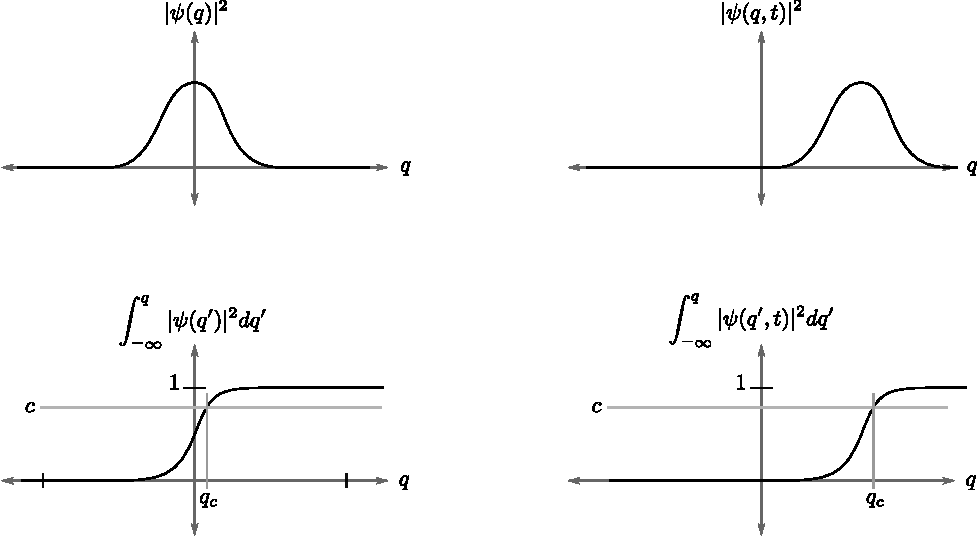
\includegraphics[width=0.95\columnwidth]{Chapter4/Figs/Vector/cingle}\caption{Illustration of the underlying principle of the continuously c-ingle
model\label{fig:Illustration-of-cingle}}
\end{figure}
and the initial state is given by a Gaussian. Now the cumulative of
this can be quickly constructed, and where the $c$ line intersects
the graph, that will yield the position of the particle. At some later
time if the Gaussian shifts (assume it had some momentum), then for
the same value of $c$, the particle's location would've moved with
the Gaussian as expected. Infact this is a general feature and can
be done for all observables, including $p$. %
\begin{comment}
Reasoning similar to the previous subsection entails that this theory
is also non-multiplicative and non-contextual.
\end{comment}
The theory is explicitly non-contextual, since values are uniquely
assigned to operators, given $\psi$ and $c$. However, one needs
more analysis to extend this to multiple particles. Once that is accomplished,
one must show that measuring the observables using the Hamiltonian
approach, would yield results consistent with those obtained from
the postulates of the theory. To show then that the theory is non-contextual,
one would be required to show that all concievable measurement schemes
would produce the same result, else, like BM, this theory wouldn't
be able to predict the values of operators with only the state and
hidden variable information. %
\begin{comment}
{[}TODO: write this section properly; the main idea is that to be
consistent with the method of measuring arbitrary observables, by
position measurements, one can't assign values in the aforesaid way.
This way, you end up with two assignments for the same observable
and have to accept eventually, that the result you get would depend
on the experiment that is performed and then there's no meaning one
can assign to an observable having a value; thus if I assign a value
to position, then effectively all my remaining freedom is lost. Thus,
one would have to restrict the theory in some, which is ok for spins,
black box the other degree of freedom, but here one can't do this.
{]}
\end{comment}
Once extended appropriately, this theory would effectively overcome
all the challenges we had for testing the continuous variable extensions
of the GHZ and contextuality tests. Predictions of observables will
be straight forward. To obtain values from BM, one had to do a detailed
analysis, for RS, evaluating values of observables other than $q$
and $p$ (even $q+p$ is hard) was hard.

We had this hunch however, that the trajectory so obtained, must be
identical to Bohmian trajectories. This infact turns out to be so.
Let us take a moment to prove this, for using the same method, one
can evalute a trajectory for the momentum also. This would be distinct
from the momentum in BM. In this case, a measurement of $\hat{p}$
yields $p$ (the assigned value), unlike in BM.
\begin{prop*}
$\dot{q}=\nabla S/m$ in a continuously c-ingle theory, for a single
particle, with one degree of freedom.\end{prop*}
\begin{proof}
Let $f$ quantify some property of a particle. To point to a particle,
we can either use the variables $c,t$ or $x,t$, since we know how
$x$ and $c$ are related. Thus, one can write $f(c,t)$ or $f(x,t)$.\footnote{If you think that the two functions should be different, then the
notation is confusing you. $f(x,t)=f(t,x)$ should help resolve. The
position of the arguments is not important, this is not like a computer
function. $f(x,t)$ is the statement that $f$ is a function of $x,t$.
That's it.} Now we have 
\[
\left[\frac{\partial f}{\partial t}\right]_{c}=\left[\frac{\partial f}{\partial t}\right]_{t}.\left[\frac{\partial q}{\partial t}\right]_{c}+\left[\frac{\partial f}{\partial t}\right]_{q},
\]
where we used $f(x,t)$ on the RHS. Note also that $\dot{q}$ refers
to the velocity of a given particle, thus it must equal $\left[\partial q/\partial t\right]{}_{c}$.
Now for $f=\int_{-\infty}^{q}\left|\psi(q')\right|^{2}dq'=c$, the
LHS disappears. Consequently, we have 
\[
\left[\frac{\partial q}{\partial t}\right]_{c}=-\left[\frac{\partial f}{\partial t}\right]_{q}/\left[\frac{\partial f}{\partial q}\right]_{t},
\]
which is in a form which can be evaluated directly from the relation
given. $\left[\partial f/\partial q\right]_{t}=\left|\psi(q,t)\right|^{2}=R^{2}$,
if $\psi=Re^{iS/\hbar}$. It is easy to show that the probability
current is given by $\nabla S/m$. Using $\left[\partial\left|\psi(q,t)\right|/\partial t\right]_{q}=-\nabla.(R^{2}\nabla S/m)$,
which is effectively the probability conservation statement, derived
from Schrodinger's equation, written in polar form, it follows that
$-\left[\partial f/\partial t\right]_{q}=R^{2}\nabla S$. Thus we
have $\dot{q}=\nabla S$ as claimed.
\end{proof}
An equation similarly for $\dot{p}$ can be obtained and an appropriate
dynamics can perhaps then be constructed. It maybe mentioned as a
remark that, quite independent of it's motivation, this scheme can
be used to compute Bohmian trajectories. It is much more efficient,
as is apparent from a comparison of the resources required between
computing an integral and the steps listed in \prettyref{sec:Bohm's-Theory,-Bohmian}.


\section{The Verdict: Contextuality vs. Non-Multiplicativity}

We have already constructed an explicit non-contextual model, which
is consistent with QM. This model we knew had to be non-multiplicative.
We will see how non-multiplicativity gives rise to what one might
confuse to mean contextuality. 

The approach is to take some compatible observables, and to construct
a `super-operator', a measurement of which can yield the values of
all of these compatible observables in a single shot. We would see
then, that the in-principle measurement outcome of observing these
compatible operators, would not be consistent. Now this one might
treat as contextuality, but according to the definition in \prettyref{sec:Peres-Mermin-Revisited},
we note that this is non-multiplicativity, as per \prettyref{sec:Multiplicativity}.

Let us construct an explicit situation and make more precise statements.
Borrowing the notation from \prettyref{sec:Multiplicativity}, imagine
\[
\hat{B}_{1}=\hat{\sigma}_{z}\otimes\hat{\mathbb{I}}=\left|00\right\rangle \left\langle 00\right|+\left|01\right\rangle \left\langle 01\right|-\left[\left|10\right\rangle \left\langle 10\right|+\left|11\right\rangle \left\langle 11\right|\right],
\]
\[
\hat{B}_{2}=\hat{\mathbb{I}}\otimes\hat{\sigma}_{z}=\left|10\right\rangle \left\langle 10\right|+\left|11\right\rangle \left\langle 11\right|-\left[\left|00\right\rangle \left\langle 00\right|+\left|01\right\rangle \left\langle 01\right|\right],
\]
while we define 
\[
\hat{C}=f(\{\hat{B}_{i}\})=0.\left|00\right\rangle \left\langle 00\right|+1.\left|01\right\rangle \left\langle 01\right|+2.\left|10\right\rangle \left\langle 10\right|+3.\left|11\right\rangle \left\langle 11\right|.
\]
$\hat{C}$ maybe viewed as a function of $\hat{B}_{1}$, $\hat{B}_{2}$
and other operators $\hat{B}_{i}$ which are constructed to obtain
a maximally commuting set. A measurement of $\hat{C}$, will collapse
the state into one of the states which are simultaneous eignkets of
$B_{1}$ and $B_{2}$. Consequently, from the observed value of $\hat{C}$,
one can deduce the values of $\hat{B}_{1}$ and $\hat{B}_{2}$. Now
consider $\sqrt{2}\left|\chi\right\rangle =\left|10\right\rangle +\left|01\right\rangle $,
for which $m_{1}(\hat{B}_{1})=1$, and $m_{1}(\hat{B}_{2})=1$, using
the discretely c-ingle theory (\prettyref{sub:Discretely-C-ingle-Theory}),
with $c<0.5$. However, $m_{1}(\hat{C})=1$, from which one can deduce
that $B_{1}$ was $+1$, while $B_{2}$ was $-1$. This property itself,
one may be tempted call contextuality, viz. the value of $B_{1}$
depends on whether it is measured alone or with the remaining $\{B_{i}\}$.
However, it must be noted that $B_{1}$ has a well defined value,
and so does $\hat{C}$. Thus by our accepted definition, there's no
contextuality. It is just that $m_{1}(\hat{C})\neq f(m_{1}(\hat{B}_{1}),m_{1}(\hat{B}_{2}),\dots)$,
viz. the theory is non-multiplicative. Note that after measuring $\hat{C}$
however, $m_{2}(\hat{B}_{1})=+1$ and $m_{2}(\hat{B}_{2})=-1$ (for
any value of $c$) consistent with those deduced by measuring $\hat{C}$.


\section{Denouement}

We have already learnt that the proof of `contextuality', infact requires
three assumptions, (1) multiplicativity, (2) non-contextuality and
(3) non-invasiveness. Here we were able to construct an explicit non-contextual
theory (for spins) which is non-multiplactive, but invasive and completely
consistent with QM. Succinctly stated, it satisfies (2) but neither
(3) nor (1), serving as a counter-example to the claim that non-contextual
hidden variable theories can't be consistent with QM. We also showed
how the theory might be misconstrued to be contextual and provided
a clarification. This is of interest because the contextuality arising
in BM from the measurement schemes, has been a source of confusion
about the said notion, arising in the PM situation.

\begin{comment}

\section{First Section of the Third Chapter}

And now I begin my third chapter here . . . And now to cite some more
people \cite{prime-number-theorem,texbook,SFPT,latex}


\subsection{First Subsection in the First Section . . .}

and some more


\subsection{Second Subsection in the First Section . . . }

and some more . . . 


\subsubsection{First subsub section in the second subsection . . . }

and some more in the first subsub section otherwise it all looks the
same doesn\textquoteright t it? well we can add some text to it .
. . 


\subsection{Third Subsection in the First Section . . . }

and some more text . . . 


\subsubsection{First subsub section in the third subsection . . . }

and some more in the first subsub section otherwise it all looks the
same doesn\textquoteright t it? well we can add some text to it and
some more and some more and some more and some more


\section{Second section with a Table}

Oh I have a table, which I can to refer (See \ref{tab:My-first-table}).

\begin{table}[H]
\hfill{}%
\begin{tabular}{|c|c|c|}
\hline 
\textbf{1} & \textbf{2} & \textbf{3}\tabularnewline
\hline 
\hline 
4 & 5 & 6\tabularnewline
\hline 
7 & 8 & 9\tabularnewline
\hline 
\end{tabular}\hfill{}

\caption{\label{tab:My-first-table}My first table (I know, it is a really
intuitive name) }
\end{table}
\end{comment}
\selectlanguage{english}%



\selectlanguage{british}%

\chapter{Epilogue}


\section{Implications}

In this section, non-contextuality (see \prettyref{sec:Peres-Mermin-Revisited})
will be assumed and notation will be borrowed from \prettyref{sec:Multiplicativity}.
We will use our understanding from multiplicativity, to investigate
it's relationship between entanglement, locality and superposition. 


\subsection{Superposition}

It is known that for simultaneous eigenstates of $\hat{B}_{i}$, multiplicativity
must hold. Consequently, any violation of multiplicativity must arise
from states that are superpositions (of the simultaneous eigenkets).
Note however, that entanglement is not necessary to show a violation,
since the PM test is a state independent test, where a separable state
can be used to arrive at a contradiction. 


\subsection{Non Locality and Entanglement}

It is known from \prettyref{sec:Bell's-Theorem} that $\left\langle \hat{B}\right\rangle \le2$,
where $\hat{B}$ is the Bell operator as defined there. If we assume
(1), (2) and (3), as given in \prettyref{sec:Peres-Mermin-Revisited},
then also it can be proven that $\left\langle \hat{B}\right\rangle \le2$.
To see this, consider $\hat{B}_{1}=\hat{a}_{1}\otimes\hat{\mathbb{I}}$
and $\hat{B}_{2}=\hat{\mathbb{I}}\otimes\hat{b}_{1}$, so that $[\hat{B}_{1},\hat{B}_{2}]=0$
and $\hat{C}\equiv\hat{B}_{1}\hat{B}_{2}$. From multiplicativity,
it follows that $m_{1}(\hat{C})=m_{1}(\hat{B}_{1})m_{1}(\hat{B}_{2})$.
This entails that $m(\hat{a}_{1}\otimes\hat{b}_{1})=m(\hat{a}_{1}\otimes\hat{\mathbb{I}})m(\hat{\mathbb{I}}\otimes\hat{b}_{1})$,
where the subscript has been suppressed for brevity. Note that $m(\hat{*})$,
will depend on the state $\left|\psi\right\rangle $ and the hidden
variables. Therefore, averaging multiple measurements, corresponds
to averaging over the hidden variables. This is expressed by $\left\langle m(\hat{a}_{1}\otimes\hat{b}_{1})\right\rangle =\left\langle m(\hat{a}_{1}\otimes\hat{\mathbb{I}})\right\rangle \left\langle m(\hat{\mathbb{I}}\otimes\hat{b}_{1})\right\rangle $.
One can repeat this argument for each term in $\left\langle \hat{B}\right\rangle $.
Using the fact that $-1\le m(\hat{*})\le1$, and that the extrema
will occur only at the extreme values of $m$, one can plugin $\pm1$
for each $\left\langle m(\hat{*})\right\rangle $ to obtain $\left\langle \hat{B}\right\rangle \le2$.
We can therefore conclude that a violation of Bell's inequality, entails
that atleast one of the three assumptions is wrong. 

One can infact try to show how a consistent (with QM) non-multiplicative
theory, must be non-local. Formally it is clear, since a violation
of Bell's inequality implies non-locality. Consequently, any consistent
completion of QM, will be non-local. More insight can be gained, although
some care is needed. The notion of compatible observables is that
commuting observables don't disturb each other and can be simultaneously
known. While the statement is not precisely stated, we only need to
note that $m_{k_{1}}(\hat{C})=m_{k_{2}}(\hat{B}_{1})m_{k_{3}}(\hat{B}_{2})$,
for $(k_{1},k_{2},k_{3})\in\{(1,2,3),(2,1,3),\dots\}$. In words,
this means that to measure $\hat{C}$, one can instead first measure
$\hat{B}_{1}$ and then measure $\hat{B}_{2}$. A multiplication of
the values obtained, can be taken to be the value a measurement of
$\hat{C}$ yields. This can be verified by measuring $\hat{C}$ subsequently.
The Bell scenario offers an interesting freedom, by restricting the
form of $\hat{B}_{i}$. To evaluate $\left\langle \hat{B}\right\rangle $,
one is required to evaluate $\left\langle \hat{B}_{1}\hat{B}_{2}\right\rangle $.
From the compatibility argument, we need to find the average value
of $m_{3}(\hat{B}_{1}\hat{B}_{2})=m_{1}(\hat{B}_{1})m_{2}(\hat{B}_{2})$,
viz. $\left\langle m_{3}(\hat{a}_{1}\otimes\hat{b}_{1})\right\rangle =\left\langle m_{1}(\hat{a}_{1}\otimes\hat{\mathbb{I}})\right\rangle \left\langle m_{2}(\hat{\mathbb{I}}\otimes\hat{b}_{1})\right\rangle $.
So far, the statements were general. Now we assume that our theory
is non-multiplicative (and non-contextual). A consistent theory (with
QM), using these assumptions, can and must violate $\left\langle \hat{B}\right\rangle \le2$.
However, if the particles are taken far away, then the only way the
theory can be non-multiplicative ($m_{1}(\hat{B}_{1})\neq m_{2}(\hat{B}_{1})$
for example), is if the theory is non-local. Locality will entail
that $m_{1}(\hat{B}_{1})=m_{2}(\hat{B}_{1})$ for instance, since
the information about which observable was measured first, can't be
propagated instantaneously. We see therefore that non-locality arises
quite naturally in consistent non-multiplicative theories.

As a remark, it maybe added that in case of the Bell Test, entanglement
is needed to show one of the three assumptions is wrong. This is so
because it can be shown that entanglement is necessary to arrive at
a violation of the inequality.


\section{Summary of Results}

Progress was made roughly in three categories, as listed. 
\begin{figure}
\begin{centering}
\includegraphics[width=0.75\columnwidth]{Chapter5/Figs/Vector/flow}
\par\end{centering}

\caption{Overview of work done during the semesters. The bold faced titles
represent new results.}
\end{figure}

\begin{itemize}
\item Bohmian Mechanics

\begin{itemize}
\item Generalized the Hamiltonian based measurement scheme to continuous
variables (see \prettyref{sub:BM-measurement-to-continuous})
\item Analytic/graphical proof of consistency check using position measurements
(see \prettyref{sub:BM-Consistency-check-measurement})
\item Analytic/graphical solution to measuring entangled spins using SG
\& using the Hamiltonian scheme (see \prettyref{sub:BM-entangled-Stern-Gerlach},
\prettyref{sub:BM-Hamiltonian-Approach-Spins})
\item Alternative proof of spins can't be associated with particles, and
must only be a property of the wavefunction (see \prettyref{sub:BM-Hamiltonian-Approach-Spins})
\item BM simulator with many trajectories (one particle, one dimensional,
arbitrary potential, see \prettyref{sec:BM-Simulator})
\end{itemize}
\item Tests of Determinism and Contextuality

\begin{itemize}
\item Optimized the phase space GHZ test (see \prettyref{sub:Optimized-Extension})
\item GHZ $\to$ a test of contextuality (see \prettyref{sub:GHZ-to-contextuality})
\item PM extension to phase space (independently re-discovered, see \prettyref{sub:Peres-Mermin-phaseSpace})
\end{itemize}
\item The Contextuality situation

\begin{itemize}
\item BM was shown consistent with PM \& restricted BM was argued to be
non-contextual (see \prettyref{sub:BM-consistent-PM})
\item `Multiplicativity' and `Sequential Multiplicativity' identified, defined
and proven where they hold (see \prettyref{sec:Multiplicativity})
\item Demonstrated `non-multiplicativity' as an alternative to contextuality,
by constructing a toy model (see \prettyref{sub:Non-Contextual-Toy-Model})
\item Proposed the `discretely c-ingle' HV theory to non-contextually explain
spins (see \prettyref{sub:Discretely-C-ingle-Theory})
\end{itemize}
\end{itemize}

\section{Conclusion}

We have shown, that atleast from the Peres Mermin's proof, it doesn't
follow that contextuality is a necessary feature of QM. We have identified
a new property, which we call non-multiplicativity. We have been able
to construct a non-contextual hidden variable theory, that is completely
consistent with QM of spins and it's predictions, we call a discretely
c-ingle theory. This theory is non-multiplicative. 

We also noted that upon restriction of measurement schemes, Bohmian
Mechanics (BM) can also be viewed as a non-contextual hidden variable
theory, which is non-multiplicative. 


\section{Digressions}

As would've been evident so far, the developments made to address
the main problem itself have not always been in the correct direction.
In addition, certain small digressions were made, some of which have
been listed for completeness.


\subsection{Cryptography using contextuality}

Interesting collaborative progress was made in developing certain
cryptography protocols using contextuality, with Jaskaran and Kishor,
who primarily constructed the schemes. A well known idea is to use
entanglement to facilitate secure sharing of keys, where the security
assurance comes from the monogomy of Bell's inequality violations.
An analogue of this idea was used, where the contextuality inequalities
are used in place of Bell's and it was found that the said method
is encouragingly secure and less resource hungry. 


\subsection{Attempt at superluminal communication with BM}

Imagine there are two particles, one with person A, and the other
with person B. Now both measure the position of their particles. Thus
the positions are precisely known. Next, they allow their particles
to evolve under a Hamiltonian (interaction) such that they become
entangled. Suppose at time $t$, the particles are entangled. Now
from the de-Broglie theory, both can predict the locations of their
particles at $t$. Now comes the interesting part. The protocol they
follow, is as follows. Say A uses this setup, only to receive signals.
If B wants to send a signal to A, all that he needs to do, is to disturb
his particle at $t$. This would cause some change in, either the
wavefunction or the position, or both, of the particle, compared to
if B had not caused any disturbance. Now A measures her particle's
position at $t+\epsilon$ and gets the value $q_{A}$. She knows what
position her particle should've been at, if B didn't do anything,
call this position $q_{A}^{(0)}$. If now $q_{A}\neq q_{A}^{(0)}$,
then she knows B sent a signal. If $q_{A}=q_{A}^{(0)}$, then she
knows nothing was sent. Since the equations are non-local, this interaction
is instantaneous, and in principle faster than speed of light.\\
Ofcourse, one can fill in the details, which is what I almost started
doing, but finding the fault in the argument is what was pivotal.
It turns out, the fault was rather straight forward, although a little
subtle. The idea is that regardless of how precise the position measurement
is, its uncertainty will spread with the wavefunction, thereby rendering
any prediction useless. Thus, in this light, chaos restores locality.
This is actually not too hard to see. Imagine you have an uncertainty
$\delta q$, when you measured the position and got the value $q$.
Now we can imagine a gaussian associated with this, as the wavefunction,
after collapse. Since the de-Broglie Bohm theory ensures that the
probability distribution $\left|\psi\right|^{2}$ is preserved by
the dynamics of the particles, as $\psi$ evolves, $\delta q$ will
increase (in case of free evolution), effectively destroying `position
information'. The idea can only be harnessed, if one can somehow decouple
the uncertainty in $q$ from the wavefunction.


\subsection{Identical Particles, an alternate approach}

One difficulty faced when we construct a statistical description of
classical particles, is the Gibbs Paradox. At its heart, is the idea
that one can always distinguish particles, on the basis of their paths.
In QM, identical particles are handled quite elegantly, by (anti-)symmetrization
of the wavefunction. In BM however, the trajectories are again well
known and one might imagine that this signals failure of BM. It so
turns out, that upon appropriately constructing the trajectory space,
invariant under permutations of particles, one is able to stay consistent
with QM and infact, able to gain further insights. 

We realized however, that since QM describes reality, only through
a combination of operators and the state, and that one can take the
view that it is the observer that is incapable of distinguishing which
particle is being looked at, therefore one can imagine that (anti-)symmetrizing
operators should yield effectively the same results as (anti-)symmetrizing
the wavefunctions.

As an illustration, consider the state $\left|\psi\right\rangle =\left|01\right\rangle $.
If this state represented bosons, then we'd have to write according
to the usual methods of QM, $\sqrt{2}\left|\psi_{\text{I}}\right\rangle =\left|01\right\rangle +\left|10\right\rangle $.
Now if we measure say $\hat{\sigma}_{z}\otimes\hat{\mathbb{I}}$,
on $\left|\psi\right\rangle $, we'd obtain $+1$, while the same
measurement on $\left|\psi_{\text{I}}\right\rangle $ would yield
$0$ (on an average, in this case). However, if we instead symmetrize
the operator as $\left(\sigma_{z}\otimes\mathbb{I}+\mathbb{I}\otimes\sigma_{z}\right)/2$,
then even if we measure $\left|\psi\right\rangle $, then on average.
We'd get $0$ upon measuring $\left|\psi_{\text{I }}\right\rangle $
also, as is expected.

I was told by Prof. Mukunda that this has been discussed earlier by
Messiah and Greenberg \cite{symmetrizationIdentical}, in the context
of particle physics. However when considered in view of the Bohmian
formalism, it might yield an interesting alternative to the problem
of identical particles.

\begin{comment}

\section{First Section of the Third Chapter}

And now I begin my third chapter here . . . And now to cite some more
people \cite{prime-number-theorem,texbook,SFPT,latex}


\subsection{First Subsection in the First Section . . .}

and some more


\subsection{Second Subsection in the First Section . . . }

and some more . . . 


\subsubsection{First subsub section in the second subsection . . . }

and some more in the first subsub section otherwise it all looks the
same doesn\textquoteright t it? well we can add some text to it .
. . 


\subsection{Third Subsection in the First Section . . . }

and some more text . . . 


\subsubsection{First subsub section in the third subsection . . . }

and some more in the first subsub section otherwise it all looks the
same doesn\textquoteright t it? well we can add some text to it and
some more and some more and some more and some more


\section{Second section with a Table}

Oh I have a table, which I can to refer (See \ref{tab:My-first-table}).

\begin{table}[H]
\hfill{}%
\begin{tabular}{|c|c|c|}
\hline 
\textbf{1} & \textbf{2} & \textbf{3}\tabularnewline
\hline 
\hline 
4 & 5 & 6\tabularnewline
\hline 
7 & 8 & 9\tabularnewline
\hline 
\end{tabular}\hfill{}

\caption{\label{tab:My-first-table}My first table (I know, it is a really
intuitive name) }
\end{table}
\end{comment}
\selectlanguage{english}%



% Back matter

\global\long\def\bibname{References}


\bibliographystyle{amsalpha}
\bibliography{References/references}


\appendix


\printindex{}
\end{document}
